% !TeX program = xelatex
% 第十六章 偏导数与全微分
\chapter{偏导数与全微分}

在一元函数的微分学中，我们引入了导数（微商）与微分的概念．导数是一个连续量随另一个连续量变化的瞬时变化率，微分则是函数改变量的线性主要部分．并且，我们证明了函数在某点可导，可微分及连续之间的关系为：
\[
\text{可导}\Leftrightarrow\text{可微分}\Rightarrow\text{连续}.
\]
对于二元函数微分学，我们同样要讨论函数的变化率和微分的概念，但由于自变量的个数不是一个，使得讨论较一元函数要复杂一些．在二元函数中，让一个自变量固定，让另一个自变量变化，这就是一元函数．考虑这个一元函数的导数，就得到偏导数（偏微商）的概念．偏导数只反映函数在坐标轴方向的变化率，并不完全反映函数在一点附近的全面变化．全微分反映的正是后者．这时偏导数存在与函数可微分的关系，不像一元函数那么简单了，这是读者要特别加以注意的．

偏导数和全微分的计算完全归结为一元函数的微商运算．复合函数的高阶偏导数的计算是本章的一个难点，原因是这时变量的关系变得更复杂了．分清变量之间的依赖关系是突破难点的关键．

本章的基本要求是概念清楚，运算熟练、准确．

\section{偏导数与全微分的概念}

\subsection{偏导数}

在二元函数 $f(x,y)$ 中将 $x$，$y$ 中的一个量固定，例如固定 $y=y_{0}$，则 $f(x,y_{0})$ 就是 $x$ 的一元函数，它在 $x_{0}$ 的导数就称为二元函数 $f(x,y)$ 在 $(x_{0},y_{0})$ 关于 $x$ 的偏导数．我们用定义把它写出来．

\begin{definition}\label{def:16-1}
设函数 $f(x,y)$ 在 $(x_{0},y_{0})$ 的某邻域有定义，令
\[
\Delta_{x}f(x_{0},y_{0})=f(x_{0}+\Delta x,y_{0})-f(x_{0},y_{0}),
\]
称为函数 $f$ 在 $(x_{0},y_{0})$ 点关于 $x$ 的偏改变量．若极限
\[
\lim_{\Delta x\to 0}\frac{\Delta_{x}f(x_{0},y_{0})}{\Delta x}=\lim_{\Delta x\to 0}\frac{f(x_{0}+\Delta x,y_{0})-f(x_{0},y_{0})}{\Delta x}
\]
存在，则称此极限值为函数 $f(x,y)$ 在 $(x_{0},y_{0})$ 点关于 $x$ 的偏导数或偏微商，记为
\[
\left.\frac{\partial f}{\partial x}\right|_{(x_{0},y_{0})}\quad\text{或}\quad f_{x}(x_{0},y_{0}).
\]
类似地，若极限
\[
\lim_{\Delta y\to 0}\frac{\Delta_{y}f(x_{0},y_{0})}{\Delta y}=\lim_{\Delta y\to 0}\frac{f(x_{0},y_{0}+\Delta y)-f(x_{0},y_{0})}{\Delta y}
\]
存在，则称此极限值为函数 $f(x,y)$ 在 $(x_{0},y_{0})$ 点关于 $y$ 的偏导数或偏微商，记为
\[
\left.\frac{\partial f}{\partial y}\right|_{(x_{0},y_{0})}\quad\text{或}\quad f_{y}(x_{0},y_{0}).
\]
\end{definition}

上述定义用符号写出来就是
\[
\left.\frac{\partial f}{\partial x}\right|_{(x_{0},y_{0})}=\frac{\dd}{\dd x}f(x,y_{0})\bigg|_{x=x_{0}},\qquad
\left.\frac{\partial f}{\partial y}\right|_{(x_{0},y_{0})}=\frac{\dd}{\dd y}f(x_{0},y)\bigg|_{y=y_{0}}.
\]
和一元函数情形相仿，若函数 $f(x,y)$ 在区域 $G$ 内每一点 $(x_{0},y_{0})$ 都存在对 $x$（或对 $y$）的偏导数，则这个偏导数也是 $(x,y)\ (\in G)$ 的函数，它是 $f(x,y)$ 在 $G$ 内对 $x$（或对 $y$）的偏导函数（简称偏导数），记为
\[
\frac{\partial f}{\partial x}\ \text{或}\ f_{x}(x,y)\qquad\left(\frac{\partial f}{\partial y}\ \text{或}\ f_{y}(x,y)\right).
\]
偏导数的几何意义：根据一元函数导数的几何意义，我们不难知道，$f_{x}(x_{0},y_{0})$ 就是曲面 $z=f(x,y)$ 与平面 $y=y_{0}$ 相交的曲线
\[
\begin{cases}
z=f(x,y),\\
y=y_{0}
\end{cases}
\]
在点 $(x_{0},y_{0})$ 的切线 $T_{x}$ 对于 $x$ 轴的斜率（图~\ref{fig:16-1}）．

\begin{figure}[htbp]
\centering
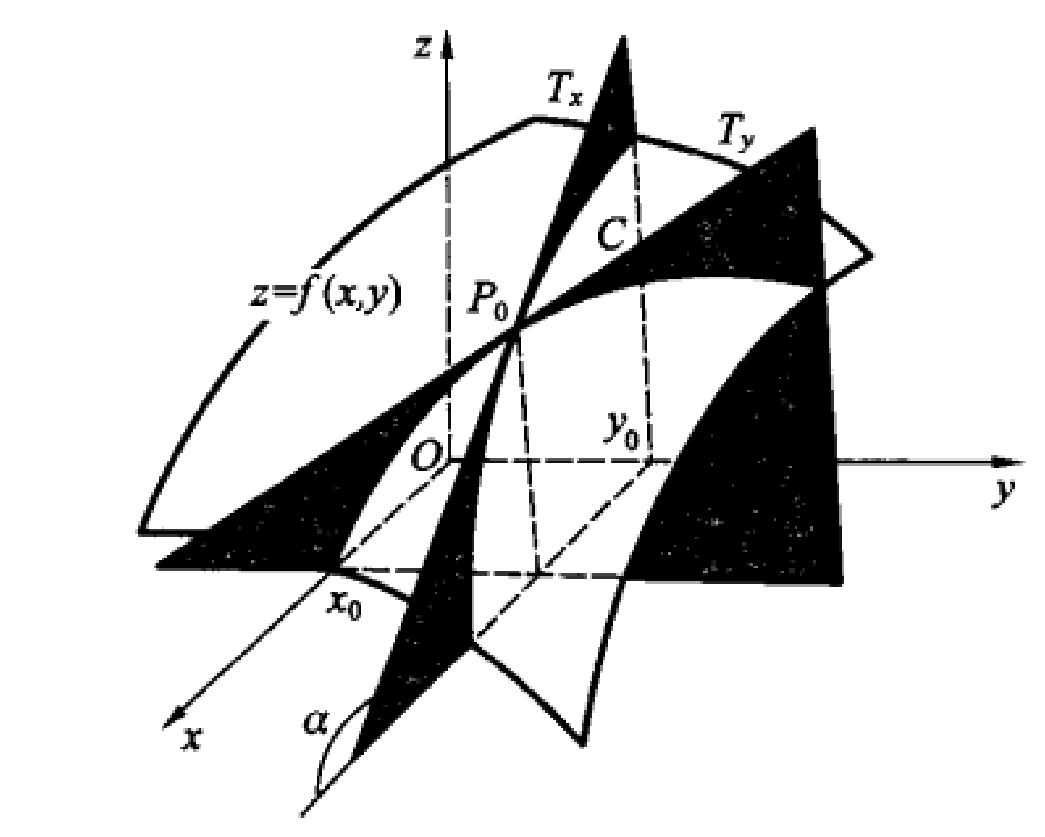
\includegraphics[width=0.5\textwidth]{work/figures/fig16-1}\caption{\relax}\label{fig:16-1}
\end{figure}

由偏导数的定义易见，求偏导数本质上归结为求一元函数的导数，只要把不相关的量视为常量即可．例如求 $f(x,y)$ 对 $x$ 的偏导数，只要把 $y$ 视为常量对 $x$ 求导即可．因此可以直接利用第四章的求导公式．

\begin{example}\label{ex:16-1-1}
设 $u=x^{y}\sin 3x$，求关于 $x$ 和 $y$ 的偏导数．
\end{example}

\begin{proof}[解]
\[
\frac{\partial u}{\partial x}=yx^{y-1}\sin 3x+3x^{y}\cos 3x,
\]
\[
\frac{\partial u}{\partial y}=x^{y}\ln x\sin 3x.
\]
\end{proof}

\begin{example}\label{ex:16-1-2}
设 $f(x,y)=\sqrt{\left|xy\right|}$，求关于 $x$ 和 $y$ 的偏导数．
\end{example}

\begin{proof}[解]
当 $x\neq 0$ 时，$f_{x}(x,y)=\dfrac{\sqrt{\left|y\right|}}{2\sqrt{\left|x\right|}}\sgn x$；

当 $y\neq 0$ 时，$f_{y}(x,y)=\dfrac{\sqrt{\left|x\right|}}{2\sqrt{\left|y\right|}}\sgn y$．

当 $x\neq 0$，$y=0$ 时，用定义求 $f_{y}$，得
\[
\lim_{\Delta y\to 0}\frac{f(x,\Delta y)-f(x,0)}{\Delta y}=\lim_{\Delta y\to 0}\frac{\sqrt{\left|x\cdot\Delta y\right|}}{\Delta y}=\infty.
\]
由此知 $f_{y}(x,0)$ 不存在 $(x\neq 0)$．同理知 $f_{x}(0,y)$ 不存在 $(y\neq 0)$．但是
\[
f_{x}(0,0)=\lim_{\Delta x\to 0}\frac{f(\Delta x,0)-f(0,0)}{\Delta x}=\lim_{\Delta x\to 0}\frac{0-0}{\Delta x}=0,
\]
\[
f_{y}(0,0)=\lim_{\Delta y\to 0}\frac{f(0,\Delta y)-f(0,0)}{\Delta y}=\lim_{\Delta y\to 0}\frac{0-0}{\Delta y}=0.
\]
综上所述：
\[
f_{x}(x,y)=\begin{cases}
\dfrac{\sqrt{\left|y\right|}}{2\sqrt{\left|x\right|}}\sgn x, & x\neq 0,\\[8pt]
\infty, & x=0,\quad y\neq 0,\\
0, & x=0,\quad y=0,
\end{cases}
\]
\[
f_{y}(x,y)=\begin{cases}
\dfrac{\sqrt{\left|x\right|}}{2\sqrt{\left|y\right|}}\sgn y, & y\neq 0,\\[8pt]
\infty, & x\neq 0,\quad y=0,\\
0, & x=0,\quad y=0.
\end{cases}
\]
\end{proof}

\begin{example}\label{ex:16-1-3}
设
\[
f(x,y)=\begin{cases}
0, & x=0\ \text{或}\ y=0,\\
1, & \text{其他}.
\end{cases}
\]
这个函数在 $(0,0)$ 点显然不连续，但
\[
f_{x}(0,0)=\lim_{\Delta x\to 0}\frac{f(\Delta x,0)-f(0,0)}{\Delta x}=\lim_{\Delta x\to 0}\frac{0-0}{\Delta x}=0.
\]
同理
\[
f_{y}(0,0)=0.
\]
也就是说，函数在原点的两个偏导数都存在，但函数在原点不连续，这在几何上是很清楚的（图~\ref{fig:16-2}）．
\end{example}

\begin{figure}[htbp]
\centering
\begin{tikzpicture}[baseline=(current bounding box.center)]
  \def\hz{1.7}
  \def\ax{1.5}
  \def\ay{2.6}
  % screen vectors: +x -> (-0.78,-0.56), +y -> (1,0), +z -> (0,1)
  \fill[gray!10,draw,thick] (0,\hz) -- ({-\ax*0.78},{\hz-\ax*0.56}) -- ({-\ax*0.78+\ay},{\hz-\ax*0.56}) -- (\ay,\hz) -- cycle;
  \fill[gray!10,draw,thick] (0,\hz) -- ({-\ax*0.78},{\hz-\ax*0.56}) -- ({-\ax*0.78-\ay},{\hz-\ax*0.56}) -- (-\ay,\hz) -- cycle;
  \fill[gray!10,draw,thick] (0,\hz) -- ({\ax*0.78},{\hz+\ax*0.56}) -- ({\ax*0.78+\ay},{\hz+\ax*0.56}) -- (\ay,\hz) -- cycle;
  \fill[gray!10,draw,thick] (0,\hz) -- ({\ax*0.78},{\hz+\ax*0.56}) -- ({\ax*0.78-\ay},{\hz+\ax*0.56}) -- (-\ay,\hz) -- cycle;
  \draw[{-Latex}] (0,0) -- (-2,-1.45) node[below left] {$x$};
  \draw[{-Latex}] (0,0) -- (3.6,0) node[below left] {$y$};
  \draw[{-Latex}] (0,-0.9) -- (0,3.2) node[left] {$z$};
  \node[below left] at (0,0) {$O$};
  \node[left] at (0,\hz) {$1$};
\end{tikzpicture}\caption{\relax}\label{fig:16-2}
\end{figure}

例~\ref{ex:16-1-3} 表明，二元函数 $f(x,y)$ 在某点的两个偏导数存在，并不能推出函数在该点连续，这与一元函数 $f(x)$ 在一点可导就连续是不同的．事实上，二元函数在几何上是曲面，而函数在一点 $(x_{0},y_{0})$ 的两个偏导数存在只说明曲面上过 $(x_{0},y_{0})$ 点的两条特殊的曲线在该点有切线，它当然不能完全反映曲面在该点的性质（如连续性）．为此，下面引入全微分的概念．

\subsection{全微分}

回忆一元函数的微分，它具有两大重要特性：微分是自变量的改变量的线性函数；微分与函数的改变量之差是比自变量的改变量更高阶的无穷小量．也就是说微分是函数改变量的线性主要部分．把它推广到二元函数，我们引出如下定义．

\begin{definition}\label{def:16-2}
设函数 $z=f(x,y)$ 在 $P_{0}(x_{0},y_{0})$ 点的某邻域有定义．若函数 $f$ 在 $P_{0}$ 点的全改变量 $\Delta z$ 可表为
\begin{equation}
\begin{aligned}
\Delta z&=f(x_{0}+\Delta x,y_{0}+\Delta y)-f(x_{0},y_{0})\\
&=A\Delta x+B\Delta y+o(\rho),
\end{aligned}
\tag{1}
\end{equation}
其中 $A$，$B$ 是与 $\Delta x$，$\Delta y$ 无关（可与 $P_{0}$ 有关）的常数，$\rho=\sqrt{(\Delta x)^{2}+(\Delta y)^{2}}$，$o(\rho)$ 是比 $\rho$ 更高阶的无穷小量，则称函数在 $P_{0}$ 点可微．并称 $A\Delta x+B\Delta y$ 为函数 $f$ 在点 $P_{0}$ 的全微分，记为
\[
\dd z\mid_{P_{0}}=A\Delta x+B\Delta y.
\]
\end{definition}

从定义可见，二元函数的全微分同一元函数的微分一样，仍然具有两大特性，即二元函数的全微分是自变量的改变量的线性函数；微分与函数的全改变量之差是比 $\rho$ 更高阶的无穷小量．综合起来说就是：二元函数的全微分是函数全改变量的线性主要部分．

下面看看二元函数 $z=f(x,y)$ 在 $(x_{0},y_{0})$ 可微的几何意义．先回忆一元函数的情形．我们知道，$y=f(x)$ 在 $x_{0}$ 可微，是说函数 $y=f(x)$ 在 $x_{0}$ 的改变量 $\Delta y=f(x_{0}+\Delta x)-f(x_{0})$ 有线性主要部分 $A\Delta x=f^{\prime}(x_{0})\Delta x$，即
\begin{equation}
\Delta y=A\Delta x+o(\Delta x)=f^{\prime}(x_{0})\Delta x+o(\Delta x).
\tag{2}
\end{equation}
记 $x=x_{0}+\Delta x$，即 $\Delta x=x-x_{0}$，则（2）可写成
\begin{equation}
f(x)-f(x_{0})=f^{\prime}(x_{0})(x-x_{0})+o(x-x_{0}),
\tag{3}
\end{equation}
或
\begin{equation}
f(x)=f(x_{0})+f^{\prime}(x_{0})(x-x_{0})+o(x-x_{0}).
\tag{4}
\end{equation}
注意 $y=f(x_{0})+f^{\prime}(x_{0})(x-x_{0})$ 是曲线 $y=f(x)$ 在 $x_{0}$ 的切线，故（3）说明，函数 $f(x)$ 在 $x_{0}$ 可微，是指曲线 $y=f(x)$ 在 $x_{0}$ 有切线存在，且曲线 $y=f(x)$ 在 $x_{0}$ 附近可用直线（切线）来逼近，其误差当 $x\to x_{0}$ 时是 $x-x_{0}$ 的高阶无穷小量（见图~\ref{fig:16-3}）．

\begin{figure}[htbp]
\centering
\begin{tikzpicture}[scale=0.85,baseline=(current bounding box.center)]
  \draw[{-Latex}] (0,0) -- (4.8,0) node[below left] {$x$};
  \draw[{-Latex}] (0.7,-0.5) -- (0.7,3.3) node[left] {$y$};
  \node[below left] at (0.7,0) {$O$};
  \coordinate (P) at (1.6,1.05);
  \coordinate (Q) at (3.7,2.65);
  \coordinate (Q') at (3.7,1.85);
  \draw[thick] (0.35,0.55) .. controls (1.2,0.9) and (2.4,1.6) .. (4.3,3.2);
  \draw[thick] (0.85,0.73) -- (4.35,2.23);
  \fill (P) circle (1.3pt) node[above left] {$P$};
  \fill (Q) circle (1.3pt) node[above right] {$Q$};
  \fill (Q') circle (1.3pt) node[right] {$Q^{\prime}$};
  \draw[dashed] (P) -- (1.6,0) node[below] {$x_{0}$};
  \draw[dashed] (Q) -- (3.7,0) node[below] {$x_{0}+\Delta x$};
  \draw[dashed] (P) -- (3.7,1.05);
  \draw[latex-latex] (3.55,1.05) -- (3.55,1.85) node[left] {$\dd y$};
  \draw[latex-latex] (3.85,1.05) -- (3.85,2.65) node[right] {$\Delta y$};
\end{tikzpicture}\caption{\relax}\label{fig:16-3}
\end{figure}

对于二元函数 $z=f(x,y)$，记 $x=x_{0}+\Delta x$，$y=y_{0}+\Delta y$，即 $\Delta x=x-x_{0}$，$\Delta y=y-y_{0}$，则公式（1）可写成
\begin{equation}
f(x,y)-f(x_{0},y_{0})=A(x-x_{0})+B(y-y_{0})+o(\rho),
\tag{5}
\end{equation}
或
\begin{equation}
f(x,y)=f(x_{0},y_{0})+A(x-x_{0})+B(y-y_{0})+o(\rho),
\tag{6}
\end{equation}
其中 $\rho=\sqrt{(x-x_{0})^{2}+(y-y_{0})^{2}}$．（6）式右边的前一部分是 $x$，$y$ 的线性函数，即
\begin{equation}
z=f(x_{0},y_{0})+A(x-x_{0})+B(y-y_{0}).
\tag{7}
\end{equation}
由解析几何的知识可知，它是一空间平面方程，且过 $(x_{0},y_{0},f(x_{0},y_{0}))$．（6）式说，这个平面与曲面 $z=f(x,y)$ 在 $(x_{0},y_{0})$ 附近之差，当 $\rho\to 0$ 时是较 $\rho$ 更高阶的无穷小量．也就是说，曲面 $z=f(x,y)$ 在 $(x_{0},y_{0},f(x_{0},y_{0}))$ 附近，与一个平面十分密切．这平面当然不是别的，正是曲面过 $(x_{0},y_{0},f(x_{0},y_{0}))$ 的切平面．可以说，函数 $f(x,y)$ 在 $(x_{0},y_{0})$ 可微，其几何意义是曲面 $z=f(x,y)$ 在 $(x_{0},y_{0},f(x_{0},y_{0}))$ 有切平面存在，全微分就是线性函数在 $(x_{0},y_{0})$ 的改变量（见图~\ref{fig:16-4}）．由此可见，全微分刻画的是函数 $f(x,y)$ 在 $(x_{0},y_{0})$ 附近的全面变化，而不像偏导数那样，只描写函数在两个特殊方向的变化．下面的定理也进一步说明这一点．

\begin{figure}[htbp]
\centering
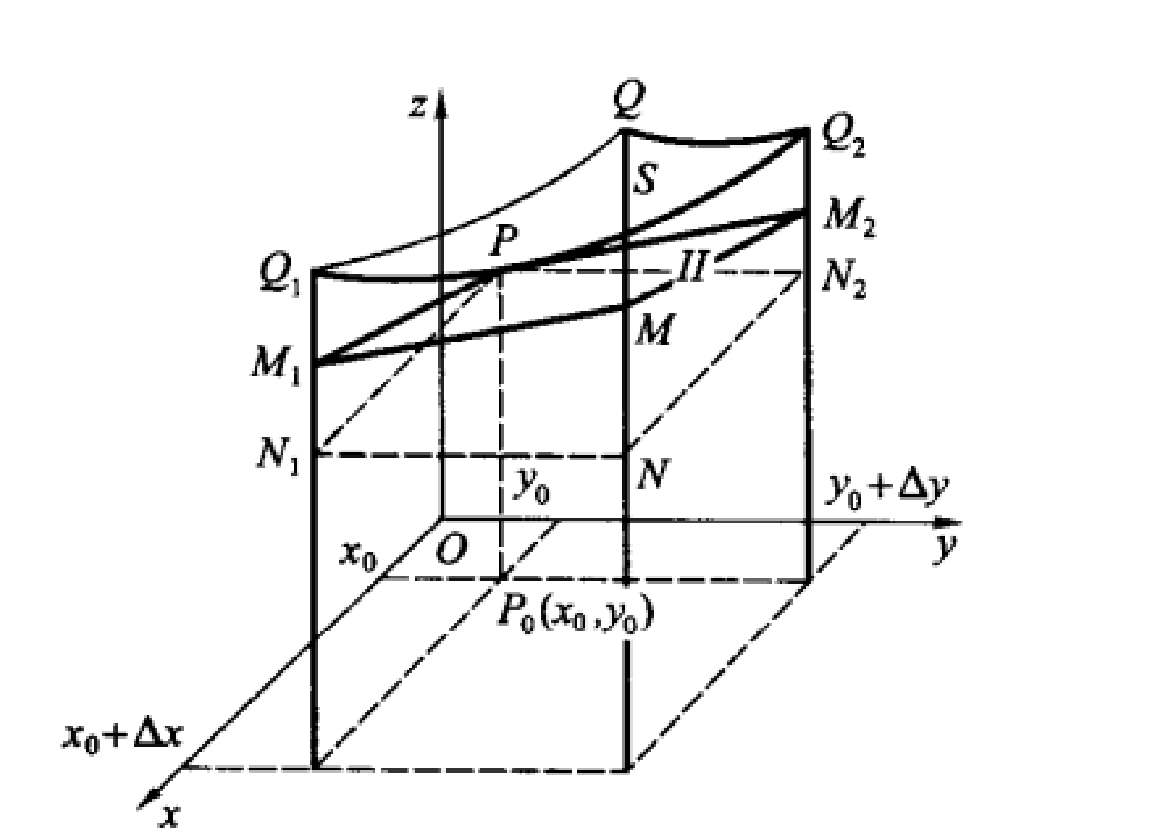
\includegraphics[width=0.55\textwidth]{work/figures/fig16-4}\caption{\relax}\label{fig:16-4}
\end{figure}

\begin{theorem}\label{thm:16-1}
若 $f(x,y)$ 在点 $P_{0}(x_{0},y_{0})$ 可微，则 $f(x,y)$ 在点 $P_{0}$ 连续．
\end{theorem}

\begin{proof}
由可微性知
\[
f(x,y)=f(x_{0},y_{0})+A(x-x_{0})+B(y-y_{0})+o(\rho),
\]
其中
\[
\rho=\sqrt{(x-x_{0})^{2}+(y-y_{0})^{2}}.
\]
令 $x\to x_{0}$，$y\to y_{0}$ 取极限，有
\[
\lim_{\substack{x\to x_{0}\\ y\to y_{0}}}f(x,y)=f(x_{0},y_{0}).
\]
这就证明了 $f(x,y)$ 在点 $P_{0}(x_{0},y_{0})$ 连续．定理~\ref{thm:16-1} 证完．
\end{proof}

\subsection{全微分与偏导数的关系}

若 $f(x,y)$ 在 $(x_{0},y_{0})$ 可微，则有
\[
\begin{aligned}
&f(x_{0}+\Delta x,y_{0}+\Delta y)-f(x_{0},y_{0})\\
={}&A\Delta x+B\Delta y+o\left(\sqrt{(\Delta x)^{2}+(\Delta y)^{2}}\right),
\end{aligned}
\]
特别地，令 $\Delta y=0$ 得
\[
f(x_{0}+\Delta x,y_{0})-f(x_{0},y_{0})=A\Delta x+o(\left|\Delta x\right|).
\]
因此
\[
\frac{f(x_{0}+\Delta x,y_{0})-f(x_{0},y_{0})}{\Delta x}=A+\frac{o(\left|\Delta x\right|)}{\Delta x}.
\]
令 $\Delta x\to 0$ 取极限，知左边的极限存在，且等于 $A$，即 $f_{x}(x_{0},y_{0})$ 存在，且
\[
A=f_{x}(x_{0},y_{0}).
\]
同理可得 $f_{y}(x_{0},y_{0})$ 存在，且
\[
B=f_{y}(x_{0},y_{0}).
\]
这样我们便证明了下面的定理．

\begin{theorem}\label{thm:16-2}
若 $z=f(x,y)$ 在点 $P_{0}(x_{0},y_{0})$ 可微，则 $f_{x}(x_{0},y_{0})$ 和 $f_{y}(x_{0},y_{0})$ 都存在，且 $f(x,y)$ 在点 $P_{0}$ 的全微分等于
\[
f_{x}(x_{0},y_{0})\Delta x+f_{y}(x_{0},y_{0})\Delta y.
\]
\end{theorem}

约定自变量的改变量等于自变量的微分，即
\[
\Delta x=\dd x,\quad \Delta y=\dd y,
\]
则 $f$ 在点 $P_{0}$ 的全微分又可写为
\[
\dd z\mid_{P_{0}}=f_{x}(x_{0},y_{0})\dd x+f_{y}(x_{0},y_{0})\dd y.
\]
若 $z=f(x,y)$ 在某区域 $G$ 上每点可微，则
\[
\dd z=f_{x}(x,y)\dd x+f_{y}(x,y)\dd y.
\]
值得指出的是，$\dd z$ 是 $x$，$y$，$\dd x$，$\dd y$ 的四元函数，对固定的 $x$，$y$，它是 $\dd x$ 与 $\dd y$ 的二元线性函数．

类似地可以定义 $n$ 元函数 $u=f(x_{1},x_{2},\cdots,x_{n})$ 的全微分，相应的公式为
\[
\dd u=\frac{\partial u}{\partial x_{1}}\dd x_{1}+\frac{\partial u}{\partial x_{2}}\dd x_{2}+\cdots+\frac{\partial u}{\partial x_{n}}\dd x_{n}.
\]
我们已经知道函数在一点的两个偏导数存在并不能推出函数在该点连续，因此，更不能推出在该点可微．不过我们有下面的定理．

\begin{theorem}\label{thm:16-3}
若函数 $u=f(x,y)$ 在 $P_{0}(x_{0},y_{0})$ 点的某邻域 $O(P_{0})$ 内存在偏导数，且 $f_{x}(x,y)$，$f_{y}(x,y)$ 在 $P_{0}$ 点连续，则 $f(x,y)$ 在 $P_{0}$ 点可微．
\end{theorem}

\begin{proof}
设 $\left|\Delta x\right|$，$\left|\Delta y\right|$ 充分小使得 $(x_{0}+\Delta x,y_{0}+\Delta y)\in O(P_{0})$．将 $\Delta f(x_{0},y_{0})$ 表为
\[
\begin{aligned}
\Delta f(x_{0},y_{0})&=f(x_{0}+\Delta x,y_{0}+\Delta y)-f(x_{0},y_{0})\\
&=\left[f(x_{0}+\Delta x,y_{0}+\Delta y)-f(x_{0}+\Delta x,y_{0})\right]\\
&\quad+\left[f(x_{0}+\Delta x,y_{0})-f(x_{0},y_{0})\right].
\end{aligned}
\]
由一元函数的微分中值定理，存在 $\theta_{1},\theta_{2}\in(0,1)$，使得
\[
\Delta f(x_{0},y_{0})=f_{y}(x_{0}+\Delta x,y_{0}+\theta_{1}\Delta y)\Delta y+f_{x}(x_{0}+\theta_{2}\Delta x,y_{0})\Delta x.
\]
由 $f_{x}$ 和 $f_{y}$ 在 $(x_{0},y_{0})$ 点连续，知
\[
\lim_{\substack{\Delta x\to 0\\ \Delta y\to 0}}f_{x}(x_{0}+\theta_{2}\Delta x,y_{0})=f_{x}(x_{0},y_{0}),
\]
\[
\lim_{\substack{\Delta x\to 0\\ \Delta y\to 0}}f_{y}(x_{0}+\Delta x,y_{0}+\theta_{1}\Delta y)=f_{y}(x_{0},y_{0}),
\]
从而有
\[
\begin{aligned}
f_{x}(x_{0}+\theta_{2}\Delta x,y_{0})&=f_{x}(x_{0},y_{0})+\alpha,\\
f_{y}(x_{0}+\Delta x,y_{0}+\theta_{1}\Delta y)&=f_{y}(x_{0},y_{0})+\beta,
\end{aligned}
\]
其中当 $\Delta x\to 0$ 且 $\Delta y\to 0$ 即 $\rho\to 0$ 时，$\alpha\to 0$，$\beta\to 0$，故
\[
\Delta f(x_{0},y_{0})=f_{x}(x_{0},y_{0})\Delta x+f_{y}(x_{0},y_{0})\Delta y+\alpha\Delta x+\beta\Delta y;
\]
而
\[
\left|\frac{\alpha\Delta x+\beta\Delta y}{\sqrt{(\Delta x)^{2}+(\Delta y)^{2}}}\right|\leqslant\left|\alpha\right|+\left|\beta\right|\to 0\quad(\rho\to 0),
\]
即 $\alpha\Delta x+\beta\Delta y=o(\rho)$．这就证明了 $f(x,y)$ 在 $P_{0}$ 可微．定理~\ref{thm:16-3} 证完．
\end{proof}

从定理证明可知，全微分定义中的（1）式等价于
\[
\Delta f(x_{0},y_{0})=A\Delta x+B\Delta y+\alpha\Delta x+\beta\Delta y,
\]
其中当 $\rho\to 0$ 时，$\alpha\to 0$，$\beta\to 0$．这个表达式有时用起来更为方便．

\begin{example}\label{ex:16-1-4}
设 $u=x^{2}y+\mathrm{e}^{xy}$，求全微分 $\dd u$．
\end{example}

\begin{proof}[解]
\[
\frac{\partial u}{\partial x}=2xy+y\mathrm{e}^{xy},
\]
\[
\frac{\partial u}{\partial y}=x^{2}+x\mathrm{e}^{xy},
\]
$\dfrac{\partial u}{\partial x}$，$\dfrac{\partial u}{\partial y}$ 都在全平面上连续，故函数在全平面上可微，且
\[
\dd u=(2xy+y\mathrm{e}^{xy})\dd x+(x^{2}+x\mathrm{e}^{xy})\dd y.
\]
\end{proof}

\begin{example}\label{ex:16-1-5}
考察函数
\[
f(x,y)=\begin{cases}
\dfrac{xy}{\sqrt{x^{2}+y^{2}}}, & x^{2}+y^{2}\neq 0,\\
0, & x^{2}+y^{2}=0
\end{cases}
\]
在原点的可微性．
\end{example}

\begin{proof}[解]
由偏导数的定义
\[
f_{x}(0,0)=\lim_{\Delta x\to 0}\frac{f(\Delta x,0)-f(0,0)}{\Delta x}=0,
\]
同理可得 $f_{y}(0,0)=0$．若函数 $f$ 在原点可微，则按可微的定义，应有
\[
\begin{aligned}
&f(\Delta x,\Delta y)-f(0,0)-\left[f_{x}(0,0)\Delta x+f_{y}(0,0)\Delta y\right]\\
={}&\frac{\Delta x\Delta y}{\sqrt{(\Delta x)^{2}+(\Delta y)^{2}}}
\end{aligned}
\]
是比 $\rho$ 更高阶的无穷小量．为此考察极限
\[
\lim_{\substack{\Delta x\to 0\\ \Delta y\to 0}}\frac{\dfrac{\Delta x\Delta y}{\sqrt{(\Delta x)^{2}+(\Delta y)^{2}}}}{\rho}=\lim_{\substack{\Delta x\to 0\\ \Delta y\to 0}}\frac{\Delta x\Delta y}{(\Delta x)^{2}+(\Delta y)^{2}}.
\]
由第十五章 §2 例 5 知，上述极限不存在，故 $f$ 在原点不可微．
\end{proof}

根据定理~\ref{thm:16-3} 我们还可知，上例中的偏导数 $f_{x}(x,y)$ 和 $f_{y}(x,y)$ 在原点必不连续．这一点也可以通过计算直接证明．事实上，
\[
f_{x}(x,y)=\begin{cases}
\dfrac{y^{3}}{\left(x^{2}+y^{2}\right)^{\frac{3}{2}}}, & x^{2}+y^{2}\neq 0,\\[6pt]
0, & x^{2}+y^{2}=0,
\end{cases}
\]
而
\[
\lim_{\substack{y=kx\\ x\to 0}}f_{x}(x,y)=\lim_{x\to 0}f_{x}(x,kx)=\lim_{x\to 0}\frac{k^{3}x^{3}}{(1+k^{2})^{\frac{3}{2}}x^{3}}=\frac{k^{3}}{(1+k^{3})^{\frac{3}{2}}}.
\]
因此 $\lim\limits_{\substack{x\to 0\\ y\to 0}}f_{x}(x,y)$ 不存在，这就证明了 $f_{x}(x,y)$ 在 $(0,0)$ 点不连续．由 $f(x,y)$ 关于 $x$、$y$ 的对称性知，$f_{y}(x,y)$ 在 $(0,0)$ 点也不连续．

请读者思考，若 $f_{x}(x,y)$ 和 $f_{y}(x,y)$ 都在 $(x_{0},y_{0})$ 点不连续，是否能推知 $f(x,y)$ 在 $(x_{0},y_{0})$ 点不可微？

最后我们把函数在某点连续、存在偏导数及可微之间的关系简单地总结如下：
\[
\text{两个偏导数都连续}\Rightarrow\text{可微}\Rightarrow\text{连续}.
\]
逆过来均不成立．

用全微分可以近似计算函数值．

\begin{example}\label{ex:16-1-6}
求 $1.08^{3.96}$ 的近似值．
\end{example}

\begin{proof}[解]
设 $f(x,y)=x^{y}$，令 $x_{0}=1$，$y_{0}=4$，$\Delta x=0.08$，$\Delta y=-0.04$，则
\[
\begin{aligned}
1.08^{3.96}&=f(x_{0}+\Delta x,y_{0}+\Delta y)\\
&\approx f(1,4)+f_{x}(1,4)\Delta x+f_{y}(1,4)\Delta y\\
&=1+4\times 0.08+(-0.04)\ln 1\\
&=1+0.32=1.32.
\end{aligned}
\]
\end{proof}

\subsection{高阶偏导数与高阶全微分}

我们先考虑二元函数 $u=f(x,y)$ 的高阶偏导数．一般说来偏导数 $f_{x}(x,y)$，$f_{y}(x,y)$ 仍是 $x$、$y$ 的函数．如果它们关于 $x$、$y$ 的偏导数存在，则称 $f_{x}(x,y)$ 和 $f_{y}(x,y)$ 关于 $x$、$y$ 的偏导数为 $f(x,y)$ 的二阶偏导数．按排列组合，二元函数的二阶偏导数有四个，分别记为
\[
\frac{\partial f_{x}}{\partial x}=\frac{\partial^{2}f}{\partial x^{2}}=f_{xx}\quad\text{或}\quad\frac{\partial^{2}u}{\partial x^{2}},
\]
\[
\frac{\partial f_{x}}{\partial y}=\frac{\partial^{2}f}{\partial x\partial y}=f_{xy}\quad\text{或}\quad\frac{\partial^{2}u}{\partial x\partial y},
\]
\[
\frac{\partial f_{y}}{\partial x}=\frac{\partial^{2}f}{\partial y\partial x}=f_{yx}\quad\text{或}\quad\frac{\partial^{2}u}{\partial y\partial x},
\]
\[
\frac{\partial f_{y}}{\partial y}=\frac{\partial^{2}f}{\partial y^{2}}=f_{yy}\quad\text{或}\quad\frac{\partial^{2}u}{\partial y^{2}}.
\]
其中 $\dfrac{\partial^{2}f}{\partial x\partial y}$ 和 $\dfrac{\partial^{2}f}{\partial y\partial x}$ 称为二阶混合偏导数．

类似地可定义三阶偏导数，如
\[
\frac{\partial}{\partial x}\left(\frac{\partial^{2}f}{\partial x^{2}}\right)=\frac{\partial^{3}f}{\partial x^{3}},
\]
\[
\frac{\partial}{\partial y}\left(\frac{\partial^{2}f}{\partial x^{2}}\right)=\frac{\partial^{3}f}{\partial x^{2}\partial y},
\]
\[
\frac{\partial}{\partial x}\left(\frac{\partial^{2}f}{\partial x\partial y}\right)=\frac{\partial^{3}f}{\partial x\partial y\partial x},
\]
等等．

\begin{example}\label{ex:16-1-7}
设 $u=x^{4}+y^{4}-4x^{3}y^{2}$，求所有二阶偏导数．
\end{example}

\begin{proof}[解]
$\dfrac{\partial u}{\partial x}=4x^{3}-12x^{2}y^{2}$，$\dfrac{\partial u}{\partial y}=4y^{3}-8x^{3}y$，
\[
\frac{\partial^{2}u}{\partial x^{2}}=12x^{2}-24xy^{2},\quad\frac{\partial^{2}u}{\partial x\partial y}=-24x^{2}y,
\]
\[
\frac{\partial^{2}u}{\partial y\partial x}=-24x^{2}y,\quad\frac{\partial^{2}u}{\partial y^{2}}=12y^{2}-8x^{3}.
\]
\end{proof}

上例中的两个混合偏导数 $\dfrac{\partial^{2}u}{\partial x\partial y}$ 和 $\dfrac{\partial^{2}u}{\partial y\partial x}$ 恰好相等，也就是说这个函数的二阶混合偏导数与对变量 $x$，$y$ 的求偏导顺序无关．我们自然要问，是否对所有的二元函数，只要两个二阶混合偏导数存在，都有 $\dfrac{\partial^{2}u}{\partial x\partial y}=\dfrac{\partial^{2}u}{\partial y\partial x}$ 呢？请看下面的例子．

\begin{example}\label{ex:16-1-8}
设
\[
f(x,y)=\begin{cases}
xy\dfrac{x^{2}-y^{2}}{x^{2}+y^{2}}, & x^{2}+y^{2}\neq 0,\\
0, & x^{2}+y^{2}=0,
\end{cases}
\]
证明 $f_{xy}(0,0)\neq f_{yx}(0,0)$．
\end{example}

\begin{proof}
由于
\[
f_{x}(x,y)=\begin{cases}
y\left(\dfrac{x^{2}-y^{2}}{x^{2}+y^{2}}+\dfrac{4x^{2}y^{2}}{(x^{2}+y^{2})^{2}}\right), & x^{2}+y^{2}\neq 0,\\
0, & x^{2}+y^{2}=0,
\end{cases}
\]
\[
f_{y}(x,y)=\begin{cases}
x\left(\dfrac{x^{2}-y^{2}}{x^{2}+y^{2}}-\dfrac{4x^{2}y^{2}}{(x^{2}+y^{2})^{2}}\right), & x^{2}+y^{2}\neq 0,\\
0, & x^{2}+y^{2}=0,
\end{cases}
\]
因此
\[
f_{xy}(0,0)=\lim_{y\to 0}\frac{f_{x}(0,y)-f_{x}(0,0)}{y}=\lim_{y\to 0}\frac{-y}{y}=-1,
\]
\[
f_{yx}(0,0)=\lim_{x\to 0}\frac{f_{y}(x,0)-f_{y}(0,0)}{x}=\lim_{x\to 0}\frac{x}{x}=1.
\]
\end{proof}

这个例子回答了上面提出的问题．两个混合偏导数都存在并不能保证它们相等．那么在什么条件下才能保证两者相等呢？下面给出一个相等的充分条件．

\begin{theorem}\label{thm:16-4}
若 $f_{xy}(x,y)$ 和 $f_{yx}(x,y)$ 在点 $(x,y)$ 都连续，则
\[
f_{xy}(x,y)=f_{yx}(x,y).
\]
\end{theorem}

\begin{proof}
先将 $f_{xy}(x,y)$ 和 $f_{yx}(x,y)$ 表成极限形式．因为
\[
f_{x}(x,y)=\lim_{\Delta x\to 0}\frac{f(x+\Delta x,y)-f(x,y)}{\Delta x},
\]
所以
\[
\begin{aligned}
&f_{xy}(x,y)\\
={}&\lim_{\Delta y\to 0}\frac{f_{x}(x,y+\Delta y)-f_{x}(x,y)}{\Delta y}\\
={}&\lim_{\Delta y\to 0}\frac{1}{\Delta y}\left[\lim_{\Delta x\to 0}\left(\frac{f(x+\Delta x,y+\Delta y)-f(x,y+\Delta y)}{\Delta x}-\frac{f(x+\Delta x,y)-f(x,y)}{\Delta x}\right)\right]\\
={}&\lim_{\Delta y\to 0}\lim_{\Delta x\to 0}\frac{f(x+\Delta x,y+\Delta y)-f(x,y+\Delta y)-f(x+\Delta x,y)+f(x,y)}{\Delta x\Delta y}.
\end{aligned}
\]
同理
\[
f_{yx}(x,y)=\lim_{\Delta x\to 0}\lim_{\Delta y\to 0}\frac{f(x+\Delta x,y+\Delta y)-f(x+\Delta x,y)-f(x,y+\Delta y)+f(x,y)}{\Delta x\Delta y}.
\]
我们发现，两个取极限的公式，其分子是相等的．因此，记
\[
\begin{aligned}
F(\Delta x,\Delta y)&=\left[f(x+\Delta x,y+\Delta y)-f(x+\Delta x,y)\right]-\\
&\quad\left[f(x,y+\Delta y)-f(x,y)\right],
\end{aligned}
\]
如果令
\[
\varphi(x)=f(x,y+\Delta y)-f(x,y),
\]
则
\[
F(\Delta x,\Delta y)=\varphi(x+\Delta x)-\varphi(x).
\]
由于 $f_{xy}(x,y)$ 在 $(x,y)$ 点连续，知 $f_{x}(x,y)$ 在 $(x,y)$ 点的某邻域存在，因此 $\varphi(x)$ 在 $x$ 点的某邻域可导．根据一元函数的微分中值定理，当 $\left|\Delta x\right|$ 充分小时，存在 $\theta_{1}\in(0,1)$，使得
\[
\begin{aligned}
F(\Delta x,\Delta y)&=\varphi^{\prime}(x+\theta_{1}\Delta x)\Delta x\\
&=\left[f_{x}(x+\theta_{1}\Delta x,y+\Delta y)-f_{x}(x+\theta_{1}\Delta x,y)\right]\Delta x.
\end{aligned}
\]
对 $y$ 再用一次微分中值定理，知存在 $\theta_{2}\in(0,1)$，使得
\begin{equation}
F(\Delta x,\Delta y)=f_{xy}(x+\theta_{1}\Delta x,y+\theta_{2}\Delta y)\Delta x\Delta y.
\tag{8}
\end{equation}
类似地，如果令
\[
\psi(y)=f(x+\Delta x,y)-f(x,y),
\]
则
\[
F(\Delta x,\Delta y)=\psi(y+\Delta y)-\psi(y).
\]
用微分中值定理，存在 $\theta_{3}\in(0,1)$，使得
\[
\begin{aligned}
F(\Delta x,\Delta y)&=\psi^{\prime}(y+\theta_{3}\Delta y)\Delta y\\
&=\left[f_{y}(x+\Delta x,y+\theta_{3}\Delta y)-f_{y}(x,y+\theta_{3}\Delta y)\right]\Delta y.
\end{aligned}
\]
再对 $x$ 用一次微分中值定理，知存在 $\theta_{4}\in(0,1)$，使得
\begin{equation}
F(\Delta x,\Delta y)=f_{yx}(x+\theta_{4}\Delta x,y+\theta_{3}\Delta y)\Delta x\Delta y.
\tag{9}
\end{equation}
比较（8）与（9），便得
\[
f_{xy}(x+\theta_{1}\Delta x,y+\theta_{2}\Delta y)=f_{yx}(x+\theta_{4}\Delta x,y+\theta_{3}\Delta y),
\]
其中 $\theta_{1}$，$\theta_{2}$，$\theta_{3}$，$\theta_{4}\in(0,1)$．令 $\Delta x\to 0$，$\Delta y\to 0$ 取极限，由两个混合偏导数都连续，知
\[
f_{xy}(x,y)=f_{yx}(x,y),
\]
定理~\ref{thm:16-4} 证完．
\end{proof}

这个定理可以推广到 $n$ 阶偏导数的情形，即若函数 $f$ 具有直到 $n$ 阶的连续偏导数，则求偏导数与变量的顺序无关．这样，二元函数 $f(x,y)$ 的 $n$ 阶偏导数就可简单地表示为
\[
\frac{\partial^{n}f}{\partial x^{k}\partial y^{n-k}},\quad k=0,1,2,\cdots,n.
\]
有了高阶偏导数，我们来定义高阶全微分．函数 $u=f(x,y)$ 的一阶全微分
\[
\dd u=f_{x}(x,y)\dd x+f_{y}(x,y)\dd y
\]
仍是 $x$，$y$ 的函数．若作为 $x$，$y$ 的函数，它是可微的，则它的全微分称为 $f(x,y)$ 的二阶全微分，这就是
\[
\begin{aligned}
\dd^{2}u&=\dd(\dd u)=\dd\left[f_{x}(x,y)\dd x\right]+\dd\left[f_{y}(x,y)\dd y\right]\\
&=\left[f_{xx}(x,y)\dd x+f_{xy}(x,y)\dd y\right]\dd x+\left[f_{yx}(x,y)\dd x+f_{yy}(x,y)\dd y\right]\dd y\\
&=f_{xx}(x,y)\dd x^{2}+\left[f_{xy}(x,y)+f_{yx}(x,y)\right]\dd x\dd y+f_{yy}(x,y)\dd y^{2}.
\end{aligned}
\]
要特别强调的是二阶全微分是一阶全微分作为 $x$，$y$ 的函数的全微分．一阶全微分依赖于四个独立的变量 $x$，$y$，$\dd x$ 和 $\dd y$，其中 $\dd x$ 和 $\dd y$ 是自变量的微分，是与 $x$，$y$ 无关的．因此求二阶全微分时，变量只有 $x$ 和 $y$，而
\[
\dd(\dd x)=\dd(\dd y)=0.
\]
当混合偏导数连续时，有
\[
\begin{aligned}
\dd^{2}u&=f_{xx}(x,y)\dd x^{2}+2f_{xy}(x,y)\dd x\dd y+f_{yy}(x,y)\dd y^{2}\\
&=\sum_{k=0}^{2}\mathrm{C}_{2}^{k}\frac{\partial^{2}f(x,y)}{\partial x^{2-k}\partial y^{k}}\dd x^{2-k}\dd y^{k}.
\end{aligned}
\]
为书写方便，我们把 $\dfrac{\partial}{\partial x}$ 和 $\dfrac{\partial}{\partial y}$ 视为算子，规定
\[
\left(\frac{\partial}{\partial x}\right)^{i}\left(\frac{\partial}{\partial y}\right)^{j}=\frac{\partial^{i+j}}{\partial x^{i}\partial y^{j}},
\]
\[
\frac{\partial^{n}}{\partial x^{n-k}\partial y^{k}}(af(x,y))=a\frac{\partial^{n}f(x,y)}{\partial x^{n-k}\partial y^{k}},\quad a\ \text{是常数},
\]
\[
\left(\frac{\partial^{n}}{\partial x^{n-k}\partial y^{k}}+\frac{\partial^{m}}{\partial x^{m-l}\partial y^{l}}\right)f(x,y)=\frac{\partial^{n}f(x,y)}{\partial x^{n-k}\partial y^{k}}+\frac{\partial^{m}f(x,y)}{\partial x^{m-l}\partial y^{l}},
\]
\[
k=0,1,2,\cdots,n,\quad l=0,1,2,\cdots,m.
\]
这时
\[
\dd^{2}u=\left(\frac{\partial}{\partial x}\dd x+\frac{\partial}{\partial y}\dd y\right)^{2}f(x,y).
\]
类似地可定义 $n$ 阶全微分为 $\dd^{n}u=\dd(\dd^{n-1}u)$．用归纳法可以证明，当 $n$ 阶偏导数连续时，有
\[
\begin{aligned}
\dd^{n}u&=\sum_{k=0}^{n}\mathrm{C}_{n}^{k}\frac{\partial^{n}f(x,y)}{\partial x^{n-k}\partial y^{k}}\dd x^{n-k}\dd y^{k}\\
&=\left(\frac{\partial}{\partial x}\dd x+\frac{\partial}{\partial y}\dd y\right)^{n}f(x,y).
\end{aligned}
\]

\begin{xiti}
\item 求下列函数的偏导数：
\begin{ziti}
\item $u=x^{2}\ln(x^{2}+y^{2})$；
\item $u=(x+y)\cos(xy)$；
\item $u=\arctan\dfrac{y}{x}$；
\item $u=xy+\dfrac{x}{y}$；
\item $u=xy\,\mathrm{e}^{\sin(xy)}$；
\item $u=x^{y}+y^{x}$．
\end{ziti}
\item 设
\[
f(x,y)=\begin{cases}
y\sin\dfrac{1}{x^{2}+y^{2}}, & x^{2}+y^{2}\neq 0,\\
0, & x^{2}+y^{2}=0.
\end{cases}
\]
考察函数在 $(0,0)$ 点的偏导数．
\item 证明函数 $u=\sqrt{x^{2}+y^{2}}$ 在 $(0,0)$ 点连续但偏导数不存在．
\item 求下列函数的全微分：
\begin{ziti}
\item $u=\sqrt{x^{2}+y^{2}+z^{2}}$；
\item $u=x\mathrm{e}^{yz}+\mathrm{e}^{-x}+y$．
\end{ziti}
\item 求下列函数在给定点的全微分：
\begin{ziti}
\item $u=\dfrac{x}{\sqrt{x^{2}+y^{2}}}$ 在点 $(1,0)$ 和 $(0,1)$；
\item $u=\ln(x+y^{2})$ 在点 $(0,1)$ 和 $(1,1)$；
\item $u=\sqrt[z]{\dfrac{x}{y}}$ 在点 $(1,1,1)$；
\item $u=x+(y-1)\arcsin\sqrt{\dfrac{x}{y}}$ 在点 $(0,1)$．
\end{ziti}
\item 考察函数 $f(x,y)$ 在 $(0,0)$ 点的可微性，其中
\[
f(x,y)=\begin{cases}
xy\sin\dfrac{1}{x^{2}+y^{2}}, & x^{2}+y^{2}\neq 0,\\
0, & x^{2}+y^{2}=0.
\end{cases}
\]
\item 证明函数
\[
f(x,y)=\begin{cases}
\dfrac{x^{2}y}{x^{2}+y^{2}}, & x^{2}+y^{2}\neq 0,\\
0, & x^{2}+y^{2}=0
\end{cases}
\]
在 $(0,0)$ 点连续且偏导数存在，但在此点不可微．
\item 证明函数
\[
f(x,y)=\begin{cases}
(x^{2}+y^{2})\sin\dfrac{1}{x^{2}+y^{2}}, & x^{2}+y^{2}\neq 0,\\
0, & x^{2}+y^{2}=0
\end{cases}
\]
的偏导数存在，但偏导数在 $(0,0)$ 点不连续，且在 $(0,0)$ 点的任何邻域中无界，而 $f$ 在原点 $(0,0)$ 可微．
\item 设
\[
f(x,y)=\begin{cases}
\dfrac{x^{2}y^{2}}{x^{2}+y^{2}}, & x^{2}+y^{2}\neq 0,\\
0, & x^{2}+y^{2}=0.
\end{cases}
\]
证明 $\dfrac{\partial f}{\partial x}$ 和 $\dfrac{\partial f}{\partial y}$ 在 $(0,0)$ 点连续．
\item 设
\[
f(x,y)=\begin{cases}
\dfrac{1-\mathrm{e}^{x(x^{2}+y^{2})}}{x^{2}+y^{2}}, & x^{2}+y^{2}\neq 0,\\
0, & x^{2}+y^{2}=0.
\end{cases}
\]
证明 $f(x,y)$ 在 $(0,0)$ 点可微，并求 $\dd f(0,0)$．
\item 设
\[
f(x,y)=\begin{cases}
\dfrac{x^{3}}{x^{2}+y^{2}}, & x^{2}+y^{2}\neq 0,\\
0, & x^{2}+y^{2}=0.
\end{cases}
\]
\begin{ziti}
\item $x=x(t)$，$y=y(t)$ 是通过原点的任意可微曲线（即 $x^{2}(0)+y^{2}(0)=0$；$t\neq 0$ 时，$x^{2}(t)+y^{2}(t)\neq 0$，$x(t)$，$y(t)$ 可微）．求证 $f(x(t),y(t))$ 可微．
\item $f(x,y)$ 在 $(0,0)$ 不可微．
\end{ziti}
\item 设 $\left|x\right|$，$\left|y\right|$ 很小，利用全微分推出下列各式的近似公式：
\begin{ziti}
\item $(1+x)^{m}(1+y)^{n}$；
\item $\arctan\dfrac{x+y}{1+xy}$．
\end{ziti}
\item 设 $u=f(x,y)$ 在矩形：$a<x<b$，$c<y<d$ 内可微，且全微分 $\dd u$ 恒为零，问 $f(x,y)$ 在该矩形内是否应取常数值？证明你的结论．
\item 设 $\dfrac{\partial f}{\partial x}$ 在 $(x_{0},y_{0})$ 存在，$\dfrac{\partial f}{\partial y}$ 在 $(x_{0},y_{0})$ 连续，求证 $f(x,y)$ 在 $(x_{0},y_{0})$ 可微．
\item 求下列函数的所有二阶偏导数：
\begin{ziti}
\item $u=\ln\sqrt{x^{2}+y^{2}}$；
\item $u=xy+\dfrac{y}{x}$；
\item $u=x\sin(x+y)+y\cos(x+y)$；
\item $u=\mathrm{e}^{xy}$．
\end{ziti}
\item 求下列函数指定阶的偏导数：
\begin{ziti}
\item $u=x^{3}\sin y+y^{3}\sin x$，求 $\dfrac{\partial^{6}u}{\partial x^{3}\partial y^{3}}$；
\item $u=\arctan\dfrac{x+y}{1-xy}$，求所有三阶偏导数；
\item $u=\sin(x^{2}+y^{2})$，求 $\dfrac{\partial^{3}u}{\partial x^{3}}$，$\dfrac{\partial^{3}u}{\partial y^{3}}$；
\item $u=xyz\,\mathrm{e}^{x+y+z}$，求 $\dfrac{\partial^{p+q+r}u}{\partial x^{p}\partial y^{q}\partial z^{r}}$；
\item $u=\dfrac{x+y}{x-y}$ $(x\neq y)$，求 $\dfrac{\partial^{m+n}u}{\partial x^{m}\partial y^{n}}$；
\item $u=\ln(ax+by)$，求 $\dfrac{\partial^{m+n}u}{\partial x^{m}\partial y^{n}}$．
\end{ziti}
\item 验证下列函数满足
\[
\frac{\partial^{2}u}{\partial x^{2}}+\frac{\partial^{2}u}{\partial y^{2}}=0.
\]
\begin{ziti}
\item $u=\ln(x^{2}+y^{2})$；
\item $u=x^{2}-y^{2}$；
\item $u=\mathrm{e}^{x}\cos y$；
\item $u=\arctan\dfrac{y}{x}$．
\end{ziti}
\item 设函数 $u=\varphi(x+\psi(y))$，证明
\[
\frac{\partial u}{\partial x}\frac{\partial^{2}u}{\partial x\partial y}=\frac{\partial u}{\partial y}\frac{\partial^{2}u}{\partial x^{2}}.
\]
\item 设 $f_{x}$，$f_{y}$ 在点 $(x_{0},y_{0})$ 的某邻域内存在且在点 $(x_{0},y_{0})$ 可微，则有
\[
f_{xy}(x_{0},y_{0})=f_{yx}(x_{0},y_{0}).
\]
\end{xiti}

\section{复合函数与隐函数微分法}

\subsection{复合函数的偏导数}

多元函数复合函数的求导法有类似于一元函数的链式法则．

\begin{theorem}\label{thm:16-5}
设 $u=f(x,y)$，而 $x=\varphi(s,t)$，$y=\psi(s,t)$．若在某点 $(s,t)$ 存在偏导数 $\dfrac{\partial x}{\partial s}$，$\dfrac{\partial x}{\partial t}$，$\dfrac{\partial y}{\partial s}$，$\dfrac{\partial y}{\partial t}$，又函数 $f$ 在 $(s,t)$ 的对应点 $(x,y)$（即点 $(x,y)=(\varphi(s,t),\psi(s,t))$）可微，则复合函数
\[
u=f(\varphi(s,t),\psi(s,t))
\]
在点 $(s,t)$ 的偏导数存在，并且
\[
\frac{\partial u}{\partial s}=\frac{\partial f}{\partial x}\frac{\partial x}{\partial s}+\frac{\partial f}{\partial y}\frac{\partial y}{\partial s},
\]
\[
\frac{\partial u}{\partial t}=\frac{\partial f}{\partial x}\frac{\partial x}{\partial t}+\frac{\partial f}{\partial y}\frac{\partial y}{\partial t}.
\]
\end{theorem}

上述公式称为求复合函数偏导数的链式法则．

\begin{proof}
我们只证明第一个公式，第二个公式的证明类似．

给 $s$ 以改变量 $\Delta s$，相应地得到 $x$ 和 $y$ 的改变量
\[
\Delta_{s}x=\varphi(s+\Delta s,t)-\varphi(s,t),
\]
\[
\Delta_{s}y=\psi(s+\Delta s,t)-\psi(s,t).
\]
由于 $f(x,y)$ 在点 $(x,y)$ 可微，有
\[
\Delta u=\frac{\partial f}{\partial x}\Delta x+\frac{\partial f}{\partial y}\Delta y+\alpha\Delta x+\beta\Delta y,
\]
其中 $\lim\limits_{\substack{\Delta x\to 0\\ \Delta y\to 0}}\alpha=\lim\limits_{\substack{\Delta x\to 0\\ \Delta y\to 0}}\beta=0$．将 $\Delta_{s}x$ 和 $\Delta_{s}y$ 代入上式中的 $\Delta x$ 与 $\Delta y$，两边除以 $\Delta s$ 便得
\[
\frac{\Delta_{s}u}{\Delta s}=\frac{\partial f}{\partial x}\frac{\Delta_{s}x}{\Delta s}+\frac{\partial f}{\partial y}\frac{\Delta_{s}y}{\Delta s}+\alpha\frac{\Delta_{s}x}{\Delta s}+\beta\frac{\Delta_{s}y}{\Delta s}.
\]
令 $\Delta s\to 0$，注意到 $\dfrac{\partial x}{\partial s}$，$\dfrac{\partial y}{\partial s}$ 存在，便得
\[
\frac{\partial u}{\partial s}=\lim_{\Delta s\to 0}\frac{\Delta_{s}u}{\Delta s}=\frac{\partial f}{\partial x}\frac{\partial x}{\partial s}+\frac{\partial f}{\partial y}\frac{\partial y}{\partial s}.
\]
定理~\ref{thm:16-5} 证完．
\end{proof}

值得指出的是，函数 $f(x,y)$ 在点 $(x,y)$ 可微的条件是不可少的．考察函数
\[
f(x,y)=\begin{cases}
\dfrac{x^{2}y}{x^{2}+y^{2}}, & x^{2}+y^{2}\neq 0,\\
0, & x^{2}+y^{2}=0.
\end{cases}
\]
令 $x=t$，$y=t$，则得复合函数
\[
u=F(t)=f(t,t)=\frac{t}{2}.
\]
于是有 $\left.\dfrac{\dd u}{\dd t}\right|_{t=0}=F^{\prime}(0)=\dfrac{1}{2}$．若用链式法则，则有
\[
\left.\frac{\dd u}{\dd t}\right|_{t=0}=\left.\frac{\partial f}{\partial x}\right|_{(0,0)}\left.\frac{\dd x}{\dd t}\right|_{t=0}+\left.\frac{\partial f}{\partial y}\right|_{(0,0)}\left.\frac{\dd y}{\dd t}\right|_{t=0}=0.
\]
可见这时链式法则不成立，原因就在于函数 $f(x,y)$ 在 $t=0$ 的对应点 $(0,0)$ 不可微（上节习题 7）．

\begin{example}\label{ex:16-2-1}
设 $u=\mathrm{e}^{x}\sin y$，$x=2st$，$y=t+s^{2}$，求 $\dfrac{\partial u}{\partial s}$，$\dfrac{\partial u}{\partial t}$．
\end{example}

\begin{proof}[解]
显然 $\dfrac{\partial u}{\partial x}=\mathrm{e}^{x}\sin y$，$\dfrac{\partial u}{\partial y}=\mathrm{e}^{x}\cos y$ 在全平面连续，从而在全平面可微，由链式法则
\[
\begin{aligned}
\frac{\partial u}{\partial s}&=\frac{\partial u}{\partial x}\frac{\partial x}{\partial s}+\frac{\partial u}{\partial y}\frac{\partial y}{\partial s}=(\mathrm{e}^{x}\sin y)(2t)+(\mathrm{e}^{x}\cos y)(2s)\\
&=2\mathrm{e}^{x}(t\sin y+s\cos y),
\end{aligned}
\]
\[
\begin{aligned}
\frac{\partial u}{\partial t}&=\frac{\partial u}{\partial x}\frac{\partial x}{\partial t}+\frac{\partial u}{\partial y}\frac{\partial y}{\partial t}=(\mathrm{e}^{x}\sin y)(2s)+(\mathrm{e}^{x}\cos y)\\
&=\mathrm{e}^{x}(2s\sin y+\cos y).
\end{aligned}
\]
\end{proof}

复合函数求偏导数的链式法则可以推广到 $m$ 个中间变量，$n$ 个自变量的情形．即若 $u=f(x_{1},x_{2},\cdots,x_{m})$ 在 $(x_{1},x_{2},\cdots,x_{m})$ 可微，$x_{k}(t_{1},t_{2},\cdots,t_{n})$ 的所有偏导数存在 $(k=1,2,\cdots,m)$，则复合函数
\[
u=f(x_{1}(t_{1},t_{2},\cdots,t_{n}),\cdots,x_{m}(t_{1},t_{2},\cdots,t_{n}))
\]
在 $(t_{1},t_{2},\cdots,t_{n})$ 的偏导数存在，且下列公式成立：
\[
\frac{\partial u}{\partial t_{i}}=\sum_{k=1}^{m}\frac{\partial f}{\partial x_{k}}\frac{\partial x_{k}}{\partial t_{i}},\quad i=1,2,\cdots,n.
\]

\begin{example}\label{ex:16-2-2}
设 $u=f(x,y,t)$，$x=\varphi(s,t)$，$y=\psi(s,t)$，求 $\dfrac{\partial u}{\partial s}$，$\dfrac{\partial u}{\partial t}$．
\end{example}

\begin{proof}[解]
这里函数有三个中间变量 $x$，$y$，$t$，两个自变量 $s$，$t$．$t$ 既是中间变量，又是自变量．由链式法则有
\[
\frac{\partial u}{\partial s}=\frac{\partial f}{\partial x}\frac{\partial\varphi}{\partial s}+\frac{\partial f}{\partial y}\frac{\partial\psi}{\partial s},
\]
\[
\frac{\partial u}{\partial t}=\frac{\partial f}{\partial x}\frac{\partial\varphi}{\partial t}+\frac{\partial f}{\partial y}\frac{\partial\psi}{\partial t}+\frac{\partial f}{\partial t}.
\]
\end{proof}

注意上面第二式中左端 $\dfrac{\partial u}{\partial t}$ 是指复合函数 $u$ 对自变量 $t$ 的偏导数，而右端第三项的 $\dfrac{\partial f}{\partial t}$ 是指函数 $f$ 作为 $x$，$y$，$t$ 的函数对 $t$ 的偏导数，或说是复合函数 $u$ 对中间变量 $t$ 的偏导数．请读者注意如何区分和如何正确地使用函数符号．

复合函数求偏导数的关键在于明确中间变量和自变量，这一点在求复合函数的高阶偏导数时显得尤为突出．我们通过举例来说明它．

\begin{example}\label{ex:16-2-3}
设 $u=f(x,y)$，$x=x(s,t)$，$y=y(s,t)$ 都有连续的二阶偏导数，求复合函数 $u(x(s,t),y(s,t))$ 的所有二阶偏导数 $\dfrac{\partial^{2}u}{\partial s^{2}}$，$\dfrac{\partial^{2}u}{\partial t^{2}}$，$\dfrac{\partial^{2}u}{\partial s\partial t}$．
\end{example}

\begin{proof}[解]
由链式法则有
\[
\begin{aligned}
\frac{\partial u}{\partial s}&=\frac{\partial f}{\partial x}\frac{\partial x}{\partial s}+\frac{\partial f}{\partial y}\frac{\partial y}{\partial s},\\
\frac{\partial u}{\partial t}&=\frac{\partial f}{\partial x}\frac{\partial x}{\partial t}+\frac{\partial f}{\partial y}\frac{\partial y}{\partial t}.
\end{aligned}
\]
在求二阶偏导数之前，先明确变量之间的关系．$\dfrac{\partial f}{\partial x}$ 和 $\dfrac{\partial f}{\partial y}$ 仍是 $x$，$y$ 的函数，而 $x$，$y$ 又是 $s$，$t$ 的函数，用下图简单地表示为：
\[
\frac{\partial f}{\partial x},\ \frac{\partial f}{\partial y}\left\{\begin{array}{l}x\left\{\begin{array}{l}s\\ t\end{array}\right.\\[4pt] y\left\{\begin{array}{l}s\\ t\end{array}\right.\end{array}\right.
\]
因此 $\dfrac{\partial f}{\partial x}$，$\dfrac{\partial f}{\partial y}$ 是中间变量为 $x$，$y$，自变量为 $s$，$t$ 的复合函数，在求 $\dfrac{\partial}{\partial s}\left(\dfrac{\partial f}{\partial x}\right)$，$\dfrac{\partial}{\partial t}\left(\dfrac{\partial f}{\partial x}\right)$，$\dfrac{\partial}{\partial s}\left(\dfrac{\partial f}{\partial y}\right)$，$\dfrac{\partial}{\partial t}\left(\dfrac{\partial f}{\partial y}\right)$ 时要再一次用链式法则．因此
\[
\frac{\partial^{2}u}{\partial s^{2}}=\frac{\partial}{\partial s}\left(\frac{\partial f}{\partial x}\right)\frac{\partial x}{\partial s}+\frac{\partial f}{\partial x}\frac{\partial^{2}x}{\partial s^{2}}+\frac{\partial}{\partial s}\left(\frac{\partial f}{\partial y}\right)\frac{\partial y}{\partial s}+\frac{\partial f}{\partial y}\frac{\partial^{2}y}{\partial s^{2}}
\]
\[
\begin{aligned}
={}&\left(\frac{\partial^{2}f}{\partial x^{2}}\frac{\partial x}{\partial s}+\frac{\partial^{2}f}{\partial x\partial y}\frac{\partial y}{\partial s}\right)\frac{\partial x}{\partial s}+\frac{\partial f}{\partial x}\frac{\partial^{2}x}{\partial s^{2}}+\left(\frac{\partial^{2}f}{\partial y\partial x}\frac{\partial x}{\partial s}+\frac{\partial^{2}f}{\partial y^{2}}\frac{\partial y}{\partial s}\right)\frac{\partial y}{\partial s}+\frac{\partial f}{\partial y}\frac{\partial^{2}y}{\partial s^{2}}\\
={}&\frac{\partial^{2}f}{\partial x^{2}}\left(\frac{\partial x}{\partial s}\right)^{2}+2\frac{\partial^{2}f}{\partial x\partial y}\frac{\partial x}{\partial s}\frac{\partial y}{\partial s}+\frac{\partial^{2}f}{\partial y^{2}}\left(\frac{\partial y}{\partial s}\right)^{2}+\frac{\partial f}{\partial x}\frac{\partial^{2}x}{\partial s^{2}}+\frac{\partial f}{\partial y}\frac{\partial^{2}y}{\partial s^{2}}.
\end{aligned}
\]
\[
\begin{aligned}
\frac{\partial^{2}u}{\partial s\partial t}&=\frac{\partial}{\partial t}\left(\frac{\partial f}{\partial x}\right)\frac{\partial x}{\partial s}+\frac{\partial f}{\partial x}\frac{\partial^{2}x}{\partial s\partial t}+\frac{\partial}{\partial t}\left(\frac{\partial f}{\partial y}\right)\frac{\partial y}{\partial s}+\frac{\partial f}{\partial y}\frac{\partial^{2}y}{\partial s\partial t}\\
&=\left(\frac{\partial^{2}f}{\partial x^{2}}\frac{\partial x}{\partial t}+\frac{\partial^{2}f}{\partial x\partial y}\frac{\partial y}{\partial t}\right)\frac{\partial x}{\partial s}+\frac{\partial f}{\partial x}\frac{\partial^{2}x}{\partial s\partial t}+\left(\frac{\partial^{2}f}{\partial y\partial x}\frac{\partial x}{\partial t}+\frac{\partial^{2}f}{\partial y^{2}}\frac{\partial y}{\partial t}\right)\frac{\partial y}{\partial s}+\frac{\partial f}{\partial y}\frac{\partial^{2}y}{\partial s\partial t}.
\end{aligned}
\]
\[
\begin{aligned}
\frac{\partial^{2}u}{\partial t^{2}}&=\frac{\partial}{\partial t}\left(\frac{\partial f}{\partial x}\right)\frac{\partial x}{\partial t}+\frac{\partial f}{\partial x}\frac{\partial^{2}x}{\partial t^{2}}+\frac{\partial}{\partial t}\left(\frac{\partial f}{\partial y}\right)\frac{\partial y}{\partial t}+\frac{\partial f}{\partial y}\frac{\partial^{2}y}{\partial t^{2}}\\
&=\left(\frac{\partial^{2}f}{\partial x^{2}}\frac{\partial x}{\partial t}+\frac{\partial^{2}f}{\partial x\partial y}\frac{\partial y}{\partial t}\right)\frac{\partial x}{\partial t}+\frac{\partial f}{\partial x}\frac{\partial^{2}x}{\partial t^{2}}+\left(\frac{\partial^{2}f}{\partial y\partial x}\frac{\partial x}{\partial t}+\frac{\partial^{2}f}{\partial y^{2}}\frac{\partial y}{\partial t}\right)\frac{\partial y}{\partial t}+\frac{\partial f}{\partial y}\frac{\partial^{2}y}{\partial t^{2}}\\
&=\frac{\partial^{2}f}{\partial x^{2}}\left(\frac{\partial x}{\partial t}\right)^{2}+2\frac{\partial^{2}f}{\partial x\partial y}\frac{\partial x}{\partial t}\frac{\partial y}{\partial t}+\frac{\partial^{2}f}{\partial y^{2}}\left(\frac{\partial y}{\partial t}\right)^{2}+\frac{\partial f}{\partial x}\frac{\partial^{2}x}{\partial t^{2}}+\frac{\partial f}{\partial y}\frac{\partial^{2}y}{\partial t^{2}}.
\end{aligned}
\]
\end{proof}

\begin{example}\label{ex:16-2-4}
设 $u=f\left(xy,\dfrac{x}{y}\right)$，求 $\dfrac{\partial u}{\partial x}$，$\dfrac{\partial^{2}u}{\partial x^{2}}$，$\dfrac{\partial^{2}u}{\partial x\partial y}$．假定所出现的一切偏导数都连续．
\end{example}

\begin{proof}[解]
令 $\xi=xy$，$\eta=\dfrac{x}{y}$．则函数 $u$ 是以 $\xi$，$\eta$ 为中间变量，$x$，$y$ 为自变量的复合函数，因此用链式法则．为了书写方便，我们常用记号
\[
f_{1}=\frac{\partial f(\xi,\eta)}{\partial\xi},\quad f_{2}=\frac{\partial f(\xi,\eta)}{\partial\eta}.
\]
因此
\[
\frac{\partial u}{\partial x}=f_{1}\frac{\partial\xi}{\partial x}+f_{2}\frac{\partial\eta}{\partial x}=yf_{1}+\frac{1}{y}f_{2}.
\]
注意到如下的函数关系：
\[
f_{1},f_{2}\left\{\begin{array}{l}\xi\left\{\begin{array}{l}x\\ y\end{array}\right.\\[4pt] \eta\left\{\begin{array}{l}x\\ y\end{array}\right.\end{array}\right.
\]
则
\[
\begin{aligned}
\frac{\partial^{2}u}{\partial x^{2}}&=y\frac{\partial}{\partial x}(f_{1})+\frac{1}{y}\frac{\partial}{\partial x}(f_{2})\\
&=y\left(f_{11}\frac{\partial\xi}{\partial x}+f_{12}\frac{\partial\eta}{\partial x}\right)+\frac{1}{y}\left(f_{21}\frac{\partial\xi}{\partial x}+f_{22}\frac{\partial\eta}{\partial x}\right)\\
&=y\left(yf_{11}+\frac{1}{y}f_{12}\right)+\frac{1}{y}\left(yf_{21}+\frac{1}{y}f_{22}\right)\\
&=y^{2}f_{11}+2f_{12}+\frac{1}{y^{2}}f_{22},
\end{aligned}
\]
\[
\begin{aligned}
\frac{\partial^{2}u}{\partial x\partial y}&=f_{1}+y\frac{\partial}{\partial y}(f_{1})-\frac{1}{y^{2}}f_{2}+\frac{1}{y}\frac{\partial}{\partial y}(f_{2})\\
&=f_{1}+y\left(f_{11}\frac{\partial\xi}{\partial y}+f_{12}\frac{\partial\eta}{\partial y}\right)-\frac{1}{y^{2}}f_{2}+\frac{1}{y}\left(f_{21}\frac{\partial\xi}{\partial y}+f_{22}\frac{\partial\eta}{\partial y}\right)\\
&=f_{1}+y\left(xf_{11}-\frac{x}{y^{2}}f_{12}\right)-\frac{1}{y^{2}}f_{2}+\frac{1}{y}\left(xf_{21}-\frac{x}{y^{2}}f_{22}\right)\\
&=xyf_{11}-\frac{x}{y^{3}}f_{22}+f_{1}-\frac{1}{y^{2}}f_{2}.
\end{aligned}
\]
\end{proof}

这里 $f_{11}$，$f_{12}=f_{21}$，$f_{22}$ 的意义自明，例如
\[
f_{11}=\frac{\partial^{2}f}{\partial\xi^{2}}.
\]
我们再举两个例子说明复合函数求偏导数的链式法则的应用．含有未知函数及其偏导数的方程称为\emph{偏微分方程}．例如
\begin{equation}
\frac{\partial^{2}u}{\partial x^{2}}+\frac{\partial^{2}u}{\partial y^{2}}+\frac{\partial^{2}u}{\partial z^{2}}=0
\tag{1}
\end{equation}
是一偏微分方程．解这个方程就是要找出函数 $u=u(x,y,z)$，把它的偏导数代入（1）成为恒等式．又如
\begin{equation}
x\,\frac{\partial z}{\partial x}+y\,\frac{\partial z}{\partial y}=xyz
\tag{2}
\end{equation}
也是偏微分方程，解这个方程就是要求出函数 $z=z(x,y)$，把它的偏导数代入（2）成为恒等式．和求解常微分方程类似，为求解偏微分方程，常常需要对自变量或因变量作代换，将方程化为易于求解的形式．

\begin{example}\label{ex:16-2-5}
对方程 $\dfrac{\partial^{2}u}{\partial t^{2}}=a^{2}\dfrac{\partial^{2}u}{\partial x^{2}}$ 作自变量的变换 $\xi=x-at$，$\eta=x+at$，将方程变换为 $u$ 关于 $\xi$，$\eta$ 的偏微分方程，然后求解．
\end{example}

\begin{proof}[解]
先明确函数关系：
\[
u\left\{\begin{array}{l}\xi\left\{\begin{array}{l}x\\ t\end{array}\right.\\[4pt] \eta\left\{\begin{array}{l}x\\ t\end{array}\right.\end{array}\right.
\]
由链式法则得
\[
\frac{\partial u}{\partial t}=\frac{\partial u}{\partial\xi}\frac{\partial\xi}{\partial t}+\frac{\partial u}{\partial\eta}\frac{\partial\eta}{\partial t}=-a\frac{\partial u}{\partial\xi}+a\frac{\partial u}{\partial\eta},
\]
\[
\begin{aligned}
\frac{\partial^{2}u}{\partial t^{2}}&=a\left(\frac{\partial^{2}u}{\partial\eta^{2}}\frac{\partial\eta}{\partial t}+\frac{\partial^{2}u}{\partial\eta\partial\xi}\frac{\partial\xi}{\partial t}\right)-a\left(\frac{\partial^{2}u}{\partial\xi^{2}}\frac{\partial\xi}{\partial t}+\frac{\partial^{2}u}{\partial\xi\partial\eta}\frac{\partial\eta}{\partial t}\right)\\
&=a^{2}\left(\frac{\partial^{2}u}{\partial\eta^{2}}+\frac{\partial^{2}u}{\partial\xi^{2}}-2\frac{\partial^{2}u}{\partial\xi\partial\eta}\right),
\end{aligned}
\]
\[
\frac{\partial u}{\partial x}=\frac{\partial u}{\partial\xi}\frac{\partial\xi}{\partial x}+\frac{\partial u}{\partial\eta}\frac{\partial\eta}{\partial x}=\frac{\partial u}{\partial\xi}+\frac{\partial u}{\partial\eta},
\]
\[
\frac{\partial^{2}u}{\partial x^{2}}=\frac{\partial^{2}u}{\partial\xi^{2}}+2\frac{\partial^{2}u}{\partial\xi\partial\eta}+\frac{\partial^{2}u}{\partial\eta^{2}}.
\]
将 $\dfrac{\partial^{2}u}{\partial t^{2}}$ 和 $\dfrac{\partial^{2}u}{\partial x^{2}}$ 代入方程得
\[
-2a^{2}\frac{\partial^{2}u}{\partial\xi\partial\eta}=2a^{2}\frac{\partial^{2}u}{\partial\xi\partial\eta},
\]
即
\begin{equation}
\frac{\partial^{2}u}{\partial\xi\partial\eta}=0.
\tag{3}
\end{equation}
把它写成
\[
\frac{\partial}{\partial\xi}\left(\frac{\partial u}{\partial\eta}\right)=0.
\]
用一元函数的微分中值定理的推论，知 $\dfrac{\partial u}{\partial\eta}$ 为一与 $\xi$ 无关的``常数''，显然这``常数''可以依赖于 $\eta$，即
\[
\frac{\partial u}{\partial\eta}=h(\eta),
\]
其中 $h(\eta)$ 是任意的可微函数．再积分一次，便得
\[
u=\int h(\eta)\dd\eta+f(\xi).
\]
同理 $f(\xi)$ 是任意的只依赖于 $\xi$ 而与 $\eta$ 无关的可微函数．由于 $h(\eta)$ 任意，等价于说 $\displaystyle\int h(\eta)\dd\eta$ 任意，记它为 $g(\eta)$，则方程（3）的``通解''为
\[
u(\xi,\eta)=f(\xi)+g(\eta),
\]
其中 $f$ 与 $g$ 是任意二次可微函数．

把变量 $\xi$，$\eta$ 变换回 $x$，$t$，便得原方程的``通解''为
\[
U(x,t)=u(x-at,x+at)=f(x-at)+g(x+at),
\]
其中 $f$ 与 $g$ 是任意二次可微函数．类似于二阶常微分方程的通解一般地包含两个任意常数，这里的二阶偏微分方程的``通解''包含了两个任意函数．
\end{proof}

\begin{example}\label{ex:16-2-6}
对方程 $y\dfrac{\partial z}{\partial x}-x\dfrac{\partial z}{\partial y}=(y-x)z$ 作自变量和因变量的代换 $u=x^{2}+y^{2}$，$v=\dfrac{1}{x}+\dfrac{1}{y}$，$w=\ln z-(x+y)$，将方程变换为 $w$ 关于 $u$，$v$ 的偏微分方程，并求解．
\end{example}

\begin{proof}[解]
由 $w=\ln z-(x+y)$ 解得 $z=\mathrm{e}^{w+x+y}$，于是函数关系可由下图表示
\[
z\left\{\begin{array}{l}w\left\{\begin{array}{l}u\left\{\begin{array}{l}x\\ y\end{array}\right.\\[4pt] v\left\{\begin{array}{l}x\\ y\end{array}\right.\end{array}\right.\\[6pt] x\\[2pt] y\end{array}\right.
\]
\[
\frac{\partial z}{\partial x}=\mathrm{e}^{w+x+y}\left(\frac{\partial w}{\partial u}\frac{\partial u}{\partial x}+\frac{\partial w}{\partial v}\frac{\partial v}{\partial x}+1\right)=z\left(2x\frac{\partial w}{\partial u}-\frac{1}{x^{2}}\frac{\partial w}{\partial v}+1\right),
\]
\[
\begin{aligned}
\frac{\partial z}{\partial y}&=\mathrm{e}^{w+x+y}\left(\frac{\partial w}{\partial u}\frac{\partial u}{\partial y}+\frac{\partial w}{\partial v}\frac{\partial v}{\partial y}+1\right)\\
&=z\left(2y\frac{\partial w}{\partial u}-\frac{1}{y^{2}}\frac{\partial w}{\partial v}+1\right).
\end{aligned}
\]
代入方程得
\[
yz\left(2x\frac{\partial w}{\partial u}-\frac{1}{x^{2}}\frac{\partial w}{\partial v}+1\right)-xz\left(2y\frac{\partial w}{\partial u}-\frac{1}{y^{2}}\frac{\partial w}{\partial v}+1\right)=(y-x)z,
\]
即
\[
z\left(\frac{x}{y^{2}}-\frac{y}{x^{2}}\right)\frac{\partial w}{\partial v}=0.
\]
由于 $\left(\dfrac{x}{y^{2}}-\dfrac{y}{x^{2}}\right)z\neq 0$，得
\[
\frac{\partial w}{\partial v}=0.
\]
因此
\[
w=f(u)=f(x^{2}+y^{2}),
\]
从而
\[
z=\mathrm{e}^{f(x^{2}+y^{2})+x+y},
\]
其中 $f$ 是任意可微函数．原来的方程只含 $z$ 的一阶偏导数，是一阶偏微分方程，它的上述``通解''也就自然只包含一个任意函数．
\end{proof}

关于偏微分方程的解法和理论，有专门的书籍讨论，我们不在此多讲了．

\subsection{复合函数的全微分}

在上一节我们已经知道函数 $u=f(x,y)$ 的全微分为
\[
\dd u=\frac{\partial f}{\partial x}\dd x+\frac{\partial f}{\partial y}\dd y.
\]
进一步若 $x=\varphi(s,t)$，$y=\psi(s,t)$，则复合函数 $u=f(\varphi(s,t),\psi(s,t))$ 作为 $s$，$t$ 的函数，其全微分为
\[
\begin{aligned}
\dd u&=\frac{\partial u}{\partial s}\dd s+\frac{\partial u}{\partial t}\dd t\\
&=\left(\frac{\partial f}{\partial x}\frac{\partial x}{\partial s}+\frac{\partial f}{\partial y}\frac{\partial y}{\partial s}\right)\dd s+\left(\frac{\partial f}{\partial x}\frac{\partial x}{\partial t}+\frac{\partial f}{\partial y}\frac{\partial y}{\partial t}\right)\dd t\\
&=\frac{\partial f}{\partial x}\left(\frac{\partial x}{\partial s}\dd s+\frac{\partial x}{\partial t}\dd t\right)+\frac{\partial f}{\partial y}\left(\frac{\partial y}{\partial s}\dd s+\frac{\partial y}{\partial t}\dd t\right)\\
&=\frac{\partial f}{\partial x}\dd x+\frac{\partial f}{\partial y}\dd y,
\end{aligned}
\]
比较上面第一个等式和最后一个等式，它们的形式是完全相同的．也就是说函数 $u$ 不论作为自变量 $s$，$t$ 的函数，还是作为中间变量 $x$，$y$ 的函数，其微分 $\dd u$ 的表达形式是一样的．这一性质称为\emph{一阶全微分形式的不变性}．它告诉我们在只含一阶微分的公式中可以任意代入变量，这和一元函数的一阶微分形式的不变性是完全一样的．

值得注意的是，在全微分
\[
\dd u=\frac{\partial f}{\partial x}\dd x+\frac{\partial f}{\partial y}\dd y
\]
中，若 $x$，$y$ 是自变量，则
\[
\dd(\dd x)=\dd^{2}x=0,\quad \dd(\dd y)=\dd^{2}y=0.
\]
但若 $x$，$y$ 是中间变量 $x=\varphi(s,t)$，$y=\psi(s,t)$，则 $\dd x$，$\dd y$ 就是函数的微分，而不是自变量的微分．一般说来，$\dd x$，$\dd y$ 是 $s$，$t$ 的函数．因此
\[
\dd(\dd x)=\dd^{2}x\neq 0,\quad \dd(\dd y)=\dd^{2}y\neq 0.
\]
故二阶全微分为
\[
\begin{aligned}
\dd^{2}u&=\dd\left(\frac{\partial f}{\partial x}\right)\dd x+\dd\left(\frac{\partial f}{\partial y}\right)\dd y+\frac{\partial f}{\partial x}\dd^{2}x+\frac{\partial f}{\partial y}\dd^{2}y\\
&=\left(\frac{\partial^{2}f}{\partial x^{2}}\dd x+\frac{\partial^{2}f}{\partial x\partial y}\dd y\right)\dd x+\left(\frac{\partial^{2}f}{\partial y\partial x}\dd x+\frac{\partial^{2}f}{\partial y^{2}}\dd y\right)\dd y+\frac{\partial f}{\partial x}\dd^{2}x+\frac{\partial f}{\partial y}\dd^{2}y\\
&=\left[\frac{\partial^{2}f}{\partial x^{2}}(\dd x)^{2}+2\frac{\partial^{2}f}{\partial x\partial y}\dd x\dd y+\frac{\partial^{2}f}{\partial y^{2}}(\dd y)^{2}\right]+\left[\frac{\partial f}{\partial x}\dd^{2}x+\frac{\partial f}{\partial y}\dd^{2}y\right].
\end{aligned}
\]
当 $x$，$y$ 不是自变量时，第二个括号不为零．可见二阶全微分对自变量和中间变量，其表达形式不再相同，因此二阶全微分不再具有形式不变性．这和一元函数的情形也是相同的．

\subsection{隐函数（组）的偏导数}

下面介绍隐函数及隐函数组的偏导数求法．这里我们总假设所求的偏导数存在，也就是说，是在这个前提下来介绍求导的方法．至于在什么条件下偏导数存在，将在下一章进行讨论．

（1）一个方程的情形

在第四章 §3，我们已经介绍过形如 $F(x,y)=0$ 的方程，如果它能确定隐函数 $y=f(x)$，并且可导，那么我们无需把 $y$ 解为 $x$ 的显函数，就能求出它的导数．事实上，只要在方程中把 $y$ 视为 $x$ 的函数，即
\[
F(x,y(x))=0,
\]
利用复合函数求导的链式法则，在方程两边对 $x$ 求导，得
\[
F_{x}+F_{y}y^{\prime}(x)=0.
\]
若 $F_{y}\neq 0$，则
\[
y^{\prime}(x)=-\frac{F_{x}(x,y)}{F_{y}(x,y)}.
\]
将这个方法进行推广．对方程 $F(x,y,z)=0$，在几何上，它是空间的曲面．假设它能确定隐函数 $z=z(x,y)$，且对 $x$ 和 $y$ 的偏导数 $\dfrac{\partial z}{\partial x}$，$\dfrac{\partial z}{\partial y}$ 都存在．为求出它们，将 $z=z(x,y)$ 代入方程得 $x$ 与 $y$ 的恒等式
\[
F(x,y,z(x,y))=0.
\]
用复合函数求偏导数的链式法则，在方程两边分别对 $x$，$y$ 求偏导数，得
\[
F_{x}+F_{z}\frac{\partial z}{\partial x}=0,
\]
\[
F_{y}+F_{z}\frac{\partial z}{\partial y}=0.
\]
若 $F_{z}\neq 0$，则
\[
\frac{\partial z}{\partial x}=-\frac{F_{x}(x,y,z)}{F_{z}(x,y,z)},\quad \frac{\partial z}{\partial y}=-\frac{F_{y}(x,y,z)}{F_{z}(x,y,z)}.
\]

\begin{example}\label{ex:16-2-7}
设 $F(xy,y+z,xz)=0$，求 $\dfrac{\partial z}{\partial x}$，$\dfrac{\partial z}{\partial y}$，$\dfrac{\partial^{2}z}{\partial x\partial y}$．
\end{example}

\begin{proof}[解]
假定方程能确定隐函数 $z=z(x,y)$，且涉及的偏导数均存在．用对复合函数求偏导数的链式法则，在方程两边分别对 $x$ 和 $y$ 求偏导数，得
\begin{equation}
F_{1}y+F_{2}\frac{\partial z}{\partial x}+F_{3}\left(z+x\frac{\partial z}{\partial x}\right)=0,
\tag{4}
\end{equation}
\begin{equation}
F_{1}x+F_{2}\left(1+\frac{\partial z}{\partial y}\right)+F_{3}x\frac{\partial z}{\partial y}=0,
\tag{5}
\end{equation}
解得
\[
\frac{\partial z}{\partial x}=-\frac{yF_{1}+zF_{3}}{F_{2}+xF_{3}},
\]
\[
\frac{\partial z}{\partial y}=-\frac{F_{2}+xF_{1}}{F_{2}+xF_{3}}.
\]
为求 $\dfrac{\partial^{2}z}{\partial x\partial y}$，在（4）式两边再对 $y$ 求偏导数，记住如下函数关系：
\[
F_{1},\ F_{2},\ F_{3}\left\{\begin{array}{l}1\left\{\begin{array}{l}x\\ y\end{array}\right.\\[4pt] 2\left\{\begin{array}{l}y\\ z\end{array}\right.\left\{\begin{array}{l}x\\ y\end{array}\right.\\[4pt] 3\left\{\begin{array}{l}x\\ z\end{array}\right.\left\{\begin{array}{l}x\\ y\end{array}\right.\end{array}\right.\qquad \frac{\partial z}{\partial x},\frac{\partial z}{\partial y}\left\{\begin{array}{l}x\\ y\end{array}\right.
\]
这时有
\[
\begin{aligned}
&F_{1}+y\left[F_{11}x+F_{12}\left(1+\frac{\partial z}{\partial y}\right)+F_{13}x\frac{\partial z}{\partial y}\right]+\\
&\frac{\partial^{2}z}{\partial x\partial y}F_{2}+\frac{\partial z}{\partial x}\left[F_{21}x+F_{22}\left(1+\frac{\partial z}{\partial y}\right)+F_{23}x\frac{\partial z}{\partial y}\right]+\\
&\left(\frac{\partial z}{\partial y}+x\frac{\partial^{2}z}{\partial x\partial y}\right)F_{3}+\left(z+x\frac{\partial z}{\partial x}\right)\left[F_{31}x+F_{32}\left(1+\frac{\partial z}{\partial y}\right)+F_{33}x\frac{\partial z}{\partial y}\right]=0,
\end{aligned}
\]
将 $\dfrac{\partial z}{\partial x}$，$\dfrac{\partial z}{\partial y}$ 代入上式，即可解出
\[
\begin{aligned}
&\frac{\partial^{2}z}{\partial x\partial y}\\
={}&\frac{-1}{\left(F_{2}+xF_{3}\right)^{3}}\left\{\left[F_{1}+y\left(xF_{11}+F_{12}\right)+z\left(xF_{31}+F_{32}\right)\right]\left(F_{2}+xF_{3}\right)^{2}-\right.\\
&\left.\left[xF_{21}+F_{22}+x\left(xF_{31}+F_{32}\right)\right]\left(yF_{1}+zF_{3}\right)\left(F_{2}+xF_{3}\right)-\right.\\
&\left.\left[y\left(F_{12}+xF_{13}\right)+F_{3}+z\left(F_{32}+xF_{33}\right)\right]\left(F_{2}+xF_{1}\right)\left(F_{2}+xF_{3}\right)+\right.\\
&\left.\left[F_{22}+xF_{23}+x\left(F_{32}+xF_{33}\right)\right]\left(yF_{1}+zF_{3}\right)\left(F_{2}+xF_{1}\right)\right\}.
\end{aligned}
\]
\end{proof}

对于更一般的方程中有 $n$ 个变量的情形，即 $F(x_{1},x_{2},\cdots,x_{n})=0$．若方程能确定隐函数 $x_{n}=f(x_{1},x_{2},\cdots,x_{n-1})$，且涉及的偏导数存在，则同样可用链式法则求得
\[
\frac{\partial f}{\partial x_{i}}=-\frac{F_{x_{i}}(x_{1},x_{2},\cdots,x_{n})}{F_{x_{n}}(x_{1},x_{2},\cdots,x_{n})},\quad i=1,2,\cdots,n-1.
\]

\begin{example}\label{ex:16-2-8}
设 $u=f(x+ut,y-ut)$，求 $\dfrac{\partial u}{\partial t}$，$\dfrac{\partial u}{\partial x}$，$\dfrac{\partial u}{\partial y}$．
\end{example}

\begin{proof}[解]
假定方程 $u=f(x+ut,y-ut)$ 可确定隐函数 $u=g(x,y,t)$，且涉及的各偏导数存在．在方程两边对 $t$ 求偏导数，得
\[
\frac{\partial u}{\partial t}=\left(u+t\frac{\partial u}{\partial t}\right)f_{1}-\left(u+t\frac{\partial u}{\partial t}\right)f_{2},
\]
解得
\[
\frac{\partial u}{\partial t}=\frac{u(f_{1}-f_{2})}{1+t(f_{2}-f_{1})}.
\]
同理在方程两边分别对 $x$ 和 $y$ 求偏导数，得
\[
\frac{\partial u}{\partial x}=\left(1+t\frac{\partial u}{\partial x}\right)f_{1}-f_{2}t\frac{\partial u}{\partial x},
\]
\[
\frac{\partial u}{\partial y}=f_{1}t\frac{\partial u}{\partial y}+\left(1-t\frac{\partial u}{\partial y}\right)f_{2},
\]
分别解得
\[
\frac{\partial u}{\partial x}=\frac{f_{1}}{1+t(f_{2}-f_{1})},
\]
\[
\frac{\partial u}{\partial y}=\frac{f_{2}}{1+t(f_{2}-f_{1})}.
\]
\end{proof}

此例若利用一阶微分形式不变性求解，会更简单．由一阶微分形式不变性有
\[
\begin{aligned}
\dd u&=f_{1}\dd(x+ut)+f_{2}\dd(y-ut)\\
&=f_{1}(\dd x+t\dd u+u\dd t)+f_{2}(\dd y-t\dd u-u\dd t),
\end{aligned}
\]
移项后得
\[
[1+t(f_{2}-f_{1})]\dd u=f_{1}\dd x+f_{2}\dd y+u(f_{1}-f_{2})\dd t,
\]
即
\[
\dd u=\frac{f_{1}\dd x+f_{2}\dd y+u(f_{1}-f_{2})\dd t}{1+t(f_{2}-f_{1})},
\]
因此
\[
\frac{\partial u}{\partial x}=\frac{f_{1}}{1+t(f_{2}-f_{1})},
\]
\[
\frac{\partial u}{\partial y}=\frac{f_{2}}{1+t(f_{2}-f_{1})},
\]
\[
\frac{\partial u}{\partial t}=\frac{u(f_{1}-f_{2})}{1+t(f_{2}-f_{1})}.
\]

（2）方程组的情形

设有方程组
\begin{equation}
\begin{cases}
F(x,y,z)=0,\\
G(x,y,z)=0.
\end{cases}
\tag{6}
\end{equation}
在几何上，它表示空间的两块曲面相交的交线，即它是一条空间曲线．因此它只有一个独立变量．不妨取 $x$ 为独立变量，则 $y$ 和 $z$ 依赖于 $x$．若存在 $D\subset\mathbf{R}$，对任意的 $x\in D$，有唯一的数对 $(y,z)\in\mathbf{R}^{2}$，使得方程组（6）成立，则说方程组（6）唯一地确定了两个隐函数（隐函数组）
\[
y=y(x),\quad z=z(x).
\]
进一步，若这两个隐函数可导，为求出 $y^{\prime}(x)$ 和 $z^{\prime}(x)$，将两个隐函数代入方程组（6），得恒等式
\begin{equation}
\begin{cases}
F(x,y(x),z(x))=0,\\
G(x,y(x),z(x))=0.
\end{cases}
\tag{7}
\end{equation}
这样方程组中每个方程左边都是 $x$ 的复合函数．在方程组（7）中两边对 $x$ 求导（设所出现的偏导数与导数存在），由链式法则得
\[
\begin{cases}
F_{x}+F_{y}y^{\prime}(x)+F_{z}z^{\prime}(x)=0,\\
G_{x}+G_{y}y^{\prime}(x)+G_{z}z^{\prime}(x)=0.
\end{cases}
\]
这是关于 $y^{\prime}(x)$ 和 $z^{\prime}(x)$ 的线性方程组．根据克拉默法则，若系数行列式
\[
\begin{vmatrix}F_{y}&F_{z}\\ G_{y}&G_{z}\end{vmatrix}\neq 0,
\]
则上述线性方程组有唯一解 $y^{\prime}(x)$，$z^{\prime}(x)$．

为书写方便，我们把上面的行列式记为
\[
\frac{\partial(F,G)}{\partial(y,z)}=\begin{vmatrix}F_{y}&F_{z}\\ G_{y}&G_{z}\end{vmatrix},
\]
并称之为函数 $F$，$G$ 关于变量 $y$，$z$ 的\emph{雅可比}（Jacobi，1804---1851）\emph{行列式}，也称为函数行列式．这样线性方程组的解可以表为
\[
\begin{aligned}
y^{\prime}(x)&=-\frac{\begin{vmatrix}F_{x}&F_{z}\\ G_{x}&G_{z}\end{vmatrix}}{\begin{vmatrix}F_{y}&F_{z}\\ G_{y}&G_{z}\end{vmatrix}}=-\frac{\dfrac{\partial(F,G)}{\partial(x,z)}}{\dfrac{\partial(F,G)}{\partial(y,z)}}=\frac{\dfrac{\partial(F,G)}{\partial(z,x)}}{\dfrac{\partial(F,G)}{\partial(y,z)}},\\
z^{\prime}(x)&=-\frac{\begin{vmatrix}F_{y}&F_{x}\\ G_{y}&G_{x}\end{vmatrix}}{\begin{vmatrix}F_{y}&F_{z}\\ G_{y}&G_{z}\end{vmatrix}}=-\frac{\dfrac{\partial(F,G)}{\partial(y,x)}}{\dfrac{\partial(F,G)}{\partial(y,z)}}=\frac{\dfrac{\partial(F,G)}{\partial(x,y)}}{\dfrac{\partial(F,G)}{\partial(y,z)}}.
\end{aligned}
\tag{8}
\]

\begin{example}\label{ex:16-2-9}
求方程组 $\begin{cases}x+y+z=0,\\ xyz=1\end{cases}$ 所确定的函数的导数 $\dfrac{\dd y}{\dd x}$，$\dfrac{\dd z}{\dd x}$，$\dfrac{\dd^{2}y}{\dd x^{2}}$．
\end{example}

\begin{proof}[解]
该方程组确定函数组 $y=y(x)$，$z=z(x)$．在方程组两边对 $x$ 求导，由复合函数求偏导数的链式法则得
\[
\begin{cases}
1+y^{\prime}+z^{\prime}=0,\\
yz+xzy^{\prime}+xyz^{\prime}=0.
\end{cases}
\]
解方程，得
\[
\begin{cases}
y^{\prime}=\dfrac{y(z-x)}{x(y-z)},\qquad\text{(9)}\\[10pt]
z^{\prime}=\dfrac{z(x-y)}{x(y-z)}.\qquad\text{(10)}
\end{cases}
\]
当然，也可以用公式（8）计算，得的结果是一样的．

为求 $y^{\prime\prime}(x)$，我们将（9）式写成
\[
(xy-xz)y^{\prime}=yz-xy,
\]
注意到 $xyz=1$，故又可写为
\[
\left(\frac{1}{z}-\frac{1}{y}\right)y^{\prime}=\frac{1}{x}-\frac{1}{z}.
\]
上式两边对 $x$ 求导，注意 $y$、$z$ 都是 $x$ 的函数，有
\[
\left(\frac{-1}{z^{2}}z^{\prime}+\frac{1}{y^{2}}y^{\prime}\right)y^{\prime}+\frac{y-z}{yz}y^{\prime\prime}=\frac{-1}{x^{2}}+\frac{1}{z^{2}}z^{\prime},
\]
将（9）、（10）两式代入上式，即得
\[
\begin{aligned}
\frac{y-z}{yz}y^{\prime\prime}&=\left(\frac{x-y}{zx(y-z)}-\frac{z-x}{yx(y-z)}\right)\frac{y(z-x)}{x(y-z)}+\left(\frac{-1}{x^{2}}+\frac{x-y}{zx(y-z)}\right)\\
&=\frac{y(x-y)-z(z-x)}{y-z}\frac{y(z-x)}{x(y-z)}+\frac{x(x-y)-z(y-z)}{x(y-z)}y\\
&=\frac{-yz\left[(z-x)^{2}+(y-z)^{2}+(x-y)^{2}\right]}{x(y-z)^{2}},
\end{aligned}
\]
从而
\[
\begin{aligned}
y^{\prime\prime}&=\frac{-(yz)^{2}\left[(z-x)^{2}+(y-z)^{2}+(x-y)^{2}\right]}{x(y-z)^{3}}\\
&=-\frac{(z-x)^{2}+(y-z)^{2}+(x-y)^{2}}{x^{3}(y-z)^{3}}.
\end{aligned}
\]
\end{proof}

\begin{example}\label{ex:16-2-10}
设 $x=r\cos\theta$，$y=r\sin\theta$，求 $\dfrac{\partial r}{\partial x}$，$\dfrac{\partial\theta}{\partial x}$，$\dfrac{\partial r}{\partial y}$，$\dfrac{\partial\theta}{\partial y}$．
\end{example}

\begin{proof}[解]
这里方程组
\begin{equation}
\begin{cases}
x=r\cos\theta,\\
y=r\sin\theta
\end{cases}
\tag{11}
\end{equation}
确定了函数组 $\begin{cases}r=r(x,y),\\ \theta=\theta(x,y).\end{cases}$ 在方程组（11）两边对 $x$ 求偏导数，有
\[
\begin{cases}
1=\dfrac{\partial r}{\partial x}\cos\theta-r\sin\theta\dfrac{\partial\theta}{\partial x},\\[6pt]
0=\dfrac{\partial r}{\partial x}\sin\theta+r\cos\theta\dfrac{\partial\theta}{\partial x}.
\end{cases}
\]
系数行列式为
\[
\begin{vmatrix}\cos\theta&-r\sin\theta\\ \sin\theta&r\cos\theta\end{vmatrix}=r,
\]
故解得
\[
\frac{\partial r}{\partial x}=\frac{1}{r}\begin{vmatrix}1&-r\sin\theta\\ 0&r\cos\theta\end{vmatrix}=\cos\theta,
\]
\[
\frac{\partial\theta}{\partial x}=\frac{1}{r}\begin{vmatrix}\cos\theta&1\\ \sin\theta&0\end{vmatrix}=-\frac{\sin\theta}{r}.
\]
方程组（10）两边再对 $y$ 求偏导数，有
\[
\begin{cases}
0=\dfrac{\partial r}{\partial y}\cos\theta-r\sin\theta\dfrac{\partial\theta}{\partial y},\\[6pt]
1=\dfrac{\partial r}{\partial y}\sin\theta+r\cos\theta\dfrac{\partial\theta}{\partial y},
\end{cases}
\]
由此解得
\[
\frac{\partial r}{\partial y}=\sin\theta,\quad \frac{\partial\theta}{\partial y}=\frac{\cos\theta}{r}.
\]
\end{proof}

用上述方法，要解两次线性方程组．若利用一阶微分形式不变性，则运算会简单许多．事实上
\[
\begin{cases}
\dd x=\cos\theta\dd r-r\sin\theta\dd\theta,\\
\dd y=\sin\theta\dd r+r\cos\theta\dd\theta,
\end{cases}
\]
这是关于 $\dd r$ 和 $\dd\theta$ 的线性方程组，解为
\[
\begin{cases}
\dd r=\cos\theta\dd x+\sin\theta\dd y,\\
\dd\theta=-\dfrac{\sin\theta}{r}\dd x+\dfrac{\cos\theta}{r}\dd y.
\end{cases}
\]
已知
\[
\dd r=\frac{\partial r}{\partial x}\dd x+\frac{\partial r}{\partial y}\dd y,
\]
\[
\dd\theta=\frac{\partial\theta}{\partial x}\dd x+\frac{\partial\theta}{\partial y}\dd y,
\]
故有
\[
\frac{\partial r}{\partial x}=\cos\theta,\quad \frac{\partial r}{\partial y}=\sin\theta,
\]
\[
\frac{\partial\theta}{\partial x}=-\frac{\sin\theta}{r},\qquad \frac{\partial\theta}{\partial y}=\frac{\cos\theta}{r}.
\]
现在只要解一次线性方程组，就可同时求出所有四个偏导数．

\begin{xiti}
\item 求下列函数的所有二阶偏导数：
\begin{ziti}
\item $u=f(ax,by)$；
\item $u=f(x+y,x-y)$；
\item $u=f(xy^{2},x^{2}y)$；
\item $u=f\left(\dfrac{x}{y},\dfrac{y}{z}\right)$；
\item $u=f(x^{2}+y^{2}+z^{2})$；
\item $u=f\left(x+y,xy,\dfrac{x}{y}\right)$．
\end{ziti}
\item 设 $z=\dfrac{y}{f(x^{2}-y^{2})}$，其中 $f$ 是可微函数，验证
\[
\frac{1}{x}\frac{\partial z}{\partial x}+\frac{1}{y}\frac{\partial z}{\partial y}=\frac{z}{y^{2}}.
\]
\item 设 $v=\dfrac{1}{r}g\left(t-\dfrac{r}{c}\right)$，$c$ 为常数，函数 $g$ 二阶可导，$r=\sqrt{x^{2}+y^{2}+z^{2}}$．证明
\[
\frac{\partial^{2}v}{\partial x^{2}}+\frac{\partial^{2}v}{\partial y^{2}}+\frac{\partial^{2}v}{\partial z^{2}}=\frac{1}{c^{2}}\frac{\partial^{2}v}{\partial t^{2}}.
\]
\item 若函数 $f(x,y,z)$ 对任意正实数 $t$ 满足关系
\[
f(tx,ty,tz)=t^{n}f(x,y,z),
\]
则称 $f(x,y,z)$ 为 $n$ 次齐次函数．设 $f(x,y,z)$ 可微，试证明 $f(x,y,z)$ 为 $n$ 次齐次函数的充要条件是
\[
x\frac{\partial f}{\partial x}+y\frac{\partial f}{\partial y}+z\frac{\partial f}{\partial z}=nf(x,y,z).
\]
\item 验证下列各式：
\begin{ziti}
\item $u=\varphi(x^{2}+y^{2})$，则 $y\dfrac{\partial u}{\partial x}-x\dfrac{\partial u}{\partial y}=0$；
\item $u=y\varphi(x^{2}-y^{2})$，则 $y\dfrac{\partial u}{\partial x}+x\dfrac{\partial u}{\partial y}=\dfrac{xu}{y}$；
\item $u=x\varphi(x+y)+y\psi(x+y)$，则 $\dfrac{\partial^{2}u}{\partial x^{2}}-2\dfrac{\partial^{2}u}{\partial x\partial y}+\dfrac{\partial^{2}u}{\partial y^{2}}=0$；
\item $u=x\varphi\left(\dfrac{y}{x}\right)+\psi\left(\dfrac{y}{x}\right)$，则 $x^{2}\dfrac{\partial^{2}u}{\partial x^{2}}+2xy\dfrac{\partial^{2}u}{\partial x\partial y}+y^{2}\dfrac{\partial^{2}u}{\partial y^{2}}=0$．
\end{ziti}
\item 设 $u=f(x,y)$ 可微，在极坐标变换
\[
x=r\cos\theta,\quad y=r\sin\theta
\]
下，证明
\[
\left(\frac{\partial u}{\partial r}\right)^{2}+\frac{1}{r^{2}}\left(\frac{\partial u}{\partial\theta}\right)^{2}=\left(\frac{\partial u}{\partial x}\right)^{2}+\left(\frac{\partial u}{\partial y}\right)^{2},
\]
\[
\frac{\partial^{2}u}{\partial r^{2}}+\frac{1}{r}\frac{\partial u}{\partial r}+\frac{1}{r^{2}}\frac{\partial^{2}u}{\partial\theta^{2}}=\frac{\partial^{2}u}{\partial x^{2}}+\frac{\partial^{2}u}{\partial y^{2}}.
\]
\item 设 $z=f(x,y)$ 可微，在坐标旋转变换
\[
x=u\cos\theta-v\sin\theta,\quad y=u\sin\theta+v\cos\theta
\]
下（其中旋转角 $\theta$ 是常数），证明
\[
\left(\frac{\partial z}{\partial x}\right)^{2}+\left(\frac{\partial z}{\partial y}\right)^{2}=\left(\frac{\partial z}{\partial u}\right)^{2}+\left(\frac{\partial z}{\partial v}\right)^{2}.
\]
这时称 $\left(\dfrac{\partial z}{\partial x}\right)^{2}+\left(\dfrac{\partial z}{\partial y}\right)^{2}$ 是一个形式不变量．
\item 设函数 $u=f(x,y)$ 满足拉普拉斯方程
\[
\frac{\partial^{2}u}{\partial x^{2}}+\frac{\partial^{2}u}{\partial y^{2}}=0,
\]
证明在下列变换下形状保持不变，即仍有 $\dfrac{\partial^{2}u}{\partial s^{2}}+\dfrac{\partial^{2}u}{\partial t^{2}}=0$．
\begin{ziti}
\item $x=\dfrac{s}{s^{2}+t^{2}}$，$y=\dfrac{t}{s^{2}+t^{2}}$；
\item $x=\mathrm{e}^{s}\cos t$，$y=\mathrm{e}^{s}\sin t$；
\item $x=\varphi(s,t)$，$y=\psi(s,t)$ 满足 $\dfrac{\partial\varphi}{\partial s}=\dfrac{\partial\psi}{\partial t}$，$\dfrac{\partial\varphi}{\partial t}=-\dfrac{\partial\psi}{\partial s}$．这组方程称为柯西--黎曼方程．
\end{ziti}
\item 作自变量的变换，取 $\xi$，$\eta$，$\zeta$ 为新的自变量：
\begin{ziti}
\item $\xi=x$，$\eta=x^{2}+y^{2}$，变换方程 $y\dfrac{\partial z}{\partial x}-x\dfrac{\partial z}{\partial y}=0$；
\item $\xi=x$，$\eta=y-x$，$\zeta=z-x$，变换方程 $\dfrac{\partial u}{\partial x}+\dfrac{\partial u}{\partial y}+\dfrac{\partial u}{\partial z}=0$．
\end{ziti}
\item 作自变量和因变量的变换，取 $u$，$v$ 为新的自变量，$w=w(u,v)$ 为新的因变量：
\begin{ziti}
\item 设 $u=x+y$，$v=\dfrac{y}{x}$，$w=\dfrac{z}{x}$，变换方程
\[
\frac{\partial^{2}z}{\partial x^{2}}-2\frac{\partial^{2}z}{\partial x\partial y}+\frac{\partial^{2}z}{\partial y^{2}}=0\text{；}
\]
\item 设 $u=\dfrac{x}{y}$，$v=x$，$w=xz-y$，变换方程
\[
y\frac{\partial^{2}z}{\partial y^{2}}+2\frac{\partial z}{\partial y}=\frac{2}{x}.
\]
\end{ziti}
\item 求下列方程所确定的函数 $z=f(x,y)$ 的一阶和二阶偏导数：
\begin{ziti}
\item $\mathrm{e}^{-xy}-2z+\mathrm{e}^{z}=0$；
\item $x+y+z=\mathrm{e}^{-(x+y+z)}$；
\item $xyz=x+y+z$；
\item $x^{2}+y^{2}+z^{2}-2x+2y-4z-5=0$．
\end{ziti}
\item 求由下列方程所确定的函数的全微分 $\dd z$：
\begin{ziti}
\item $z=f(xz,z-y)$；
\item $F(x-y,y-z,z-x)=0$；
\item $f(x+y+z,x^{2}+y^{2}+z^{2})=0$；
\item $f(x,y)+g(y,z)=0$．
\end{ziti}
\item 设 $z=z(x,y)$ 由方程
\[
x^{2}+y^{2}+z^{2}=yf\left(\frac{z}{y}\right)
\]
所确定．证明
\[
\left(x^{2}-y^{2}-z^{2}\right)\frac{\partial z}{\partial x}+2xy\frac{\partial z}{\partial y}=2xz.
\]
\item 设 $z=x^{2}+y^{2}$，其中 $y=f(x)$ 为由方程 $x^{2}-xy+y^{2}=1$ 所确定的隐函数，求 $\dfrac{\dd z}{\dd x}$ 和 $\dfrac{\dd^{2}z}{\dd x^{2}}$．
\item 设 $u=x^{2}+y^{2}+z^{2}$，其中 $z=f(x,y)$ 为由方程 $x^{3}+y^{3}+z^{3}=3xyz$ 所确定的隐函数，求 $\dfrac{\partial u}{\partial x}$，$\dfrac{\partial^{2}u}{\partial x^{2}}$．
\item 求下列方程组所确定的函数的导数或偏导数：
\begin{ziti}
\item $\left\{\begin{array}{l}x^{2}+y^{2}+z^{2}=a^{2},\\ x^{2}+y^{2}=ax,\end{array}\right.$ 求 $\dfrac{\dd y}{\dd x}$，$\dfrac{\dd z}{\dd x}$；
\item $\left\{\begin{array}{l}x-u^{2}-yv=0,\\ y-v^{2}-xu=0,\end{array}\right.$ 求 $\dfrac{\partial u}{\partial x}$，$\dfrac{\partial v}{\partial x}$，$\dfrac{\partial u}{\partial y}$，$\dfrac{\partial v}{\partial y}$；
\item $\left\{\begin{array}{l}u^{2}-v=3x+y,\\ u-2v^{2}=x-2y,\end{array}\right.$ 求 $\dfrac{\partial u}{\partial x}$，$\dfrac{\partial u}{\partial y}$，$\dfrac{\partial v}{\partial x}$，$\dfrac{\partial v}{\partial y}$；
\item $\left\{\begin{array}{l}u=xyz,\\ x^{2}+y^{2}+z^{2}=1,\end{array}\right.$ 求 $\dfrac{\partial^{2}u}{\partial x^{2}}$，$\dfrac{\partial^{2}u}{\partial y^{2}}$，$\dfrac{\partial^{2}u}{\partial x\partial y}$．
\end{ziti}
\item 下列方程组定义 $z$ 为 $x$，$y$ 的函数，求 $\dfrac{\partial z}{\partial x}$，$\dfrac{\partial z}{\partial y}$．
\begin{ziti}
\item $\left\{\begin{array}{l}x=\cos\theta\cos\varphi,\\ y=\cos\theta\sin\varphi,\\ z=\sin\theta;\end{array}\right.$
\item $\left\{\begin{array}{l}x=u+v,\\ y=u^{2}+v^{2},\\ z=u^{3}+v^{3}.\end{array}\right.$
\end{ziti}
\end{xiti}

\section{几何应用}

本节我们将利用偏导数来确定空间曲线的切向量和空间曲面的法向量．在这里，复合函数求导法和隐函数（组）求导法是强有力的工具．

在本节中我们假定所涉及的导数和偏导数总是存在的．

\subsection{空间曲线的切线与法平面}

求空间曲线的切线与法平面，关键在于求曲线的切向量 $\bm{\tau}$．若已知曲线上一点 $(x_{0},y_{0},z_{0})$ 处的切向量为
\[
\bm{\tau}(x_{0},y_{0},z_{0})=(A,B,C),
\]
则曲线在该点的切线方程为
\[
\frac{x-x_{0}}{A}=\frac{y-y_{0}}{B}=\frac{z-z_{0}}{C},
\]
曲线在该点的法平面方程为
\[
A(x-x_{0})+B(y-y_{0})+C(z-z_{0})=0.
\]
因此下面我们只讨论如何求曲线的切向量 $\bm{\tau}$．

设曲线由参数方程给出：
\[
L\colon x=x(t),\ y=y(t),\ z=z(t),\ \alpha\leqslant t\leqslant\beta.
\]
曲线上一点 $P(x_{0},y_{0},z_{0})$ 处的切线定义为过 $P$ 点的割线 $PQ$ 当 $Q$ 点沿曲线趋于 $P$ 点时的极限位置（图~\ref{fig:16-5}）．设 $t=t_{0}$ 时对应曲线上的 $P$ 点，即 $P$ 点的坐标为 $P(x(t_{0}),y(t_{0}),z(t_{0}))$，而 $Q$ 点的坐标为 $Q(x(t),y(t),z(t))$．于是割线 $PQ$ 作为向量可写成
\[
(x(t)-x(t_{0}),y(t)-y(t_{0}),z(t)-z(t_{0})),
\]
它平行于
\[
\left(\frac{x(t)-x(t_{0})}{t-t_{0}},\frac{y(t)-y(t_{0})}{t-t_{0}},\frac{z(t)-z(t_{0})}{t-t_{0}}\right),
\]

\begin{figure}[htbp]
\centering
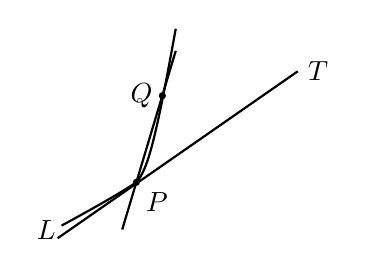
\begin{tikzpicture}[baseline=(current bounding box.center)]
  \coordinate (P) at (1.0,1.05);
  \coordinate (Q) at (1.33,2.15);
  % curve L through P
  \draw[thick] (0.05,0.5) .. controls (0.6,0.8) and (0.85,0.95) .. (P)
    .. controls (1.15,1.22) and (1.25,1.62) .. (1.5,3.0);
  % tangent at P
  \draw[thick] (0.0,0.34) -- (3.05,2.46) node[right] {$T$};
  % secant PQ
  \draw[thick] (0.82,0.45) -- (1.5,2.72);
  \fill (P) circle (1.3pt) node[below right] {$P$};
  \fill (Q) circle (1.3pt) node[left] {$Q$};
  \node[left] at (0.1,0.45) {$L$};
\end{tikzpicture}\caption{\relax}\label{fig:16-5}
\end{figure}

令 $t\to t_{0}$ 取极限，这时 $Q$ 趋于 $P$ 点，于是割线就变成为切线，从而割线上的向量就趋于切向量．故曲线在 $P$ 点的切向量为
\begin{equation}
\bm{\tau}=\pm\left(x^{\prime}(t_{0}),y^{\prime}(t_{0}),z^{\prime}(t_{0})\right).
\tag{1}
\end{equation}
特别地，若曲线 $L$ 由方程
\[
y=y(x),\ z=z(x),\ a\leqslant x\leqslant b
\]
给出，则这时可视 $x$ 为参数，即有参数方程
\[
L\colon\ x=x,\quad y=y(x),\quad z=z(x),\quad a\leqslant x\leqslant b.
\]
当 $x=x_{0}$ 时，记 $y_{0}=y(x_{0})$，$z_{0}=z(x_{0})$，这时由（1）式，曲线在 $P(x_{0},y_{0},z_{0})$ 点的切向量可取为
\begin{equation}
\bm{\tau}=\pm\left(1,y^{\prime}(x_{0}),z^{\prime}(x_{0})\right).
\tag{2}
\end{equation}
更一般地，若曲线用两曲面的交线给出
\[
L\colon\begin{cases}
F(x,y,z)=0,\\
G(x,y,z)=0,
\end{cases}
\]
$P(x_{0},y_{0},z_{0})$ 是曲线 $L$ 上的点．设上述方程组在 $P$ 点的某邻域内能确定函数组 $y=y(x)$，$z=z(x)$ 满足 $y_{0}=y(x_{0})$，$z_{0}=z(x_{0})$，且 $y^{\prime}(x)$ 和 $z^{\prime}(x)$ 存在，则由（2）式，只要求出 $y^{\prime}(x_{0})$ 和 $z^{\prime}(x_{0})$ 便可得到曲线在 $P$ 点的切向量．由隐函数组求导法，在方程两边对 $x$ 求导数，得
\[
\begin{cases}
F_{x}+F_{y}y^{\prime}+F_{z}z^{\prime}=0,\\
G_{x}+G_{y}y^{\prime}+G_{z}z^{\prime}=0.
\end{cases}
\]
当雅可比行列式 $\left.\dfrac{\partial(F,G)}{\partial(y,z)}\right|_{P}\neq 0$ 时，解得
\[
y^{\prime}(x_{0})=\left.\frac{\dfrac{\partial(F,G)}{\partial(z,x)}}{\dfrac{\partial(F,G)}{\partial(y,z)}}\right|_{P},\quad z^{\prime}(x_{0})=\left.\frac{\dfrac{\partial(F,G)}{\partial(x,y)}}{\dfrac{\partial(F,G)}{\partial(y,z)}}\right|_{P},
\]
代入（2）式得曲线在 $P(x_{0},y_{0},z_{0})$ 点的切向量
\[
\bm{\tau}=\pm\left(1,\ \frac{\dfrac{\partial(F,G)}{\partial(z,x)}}{\dfrac{\partial(F,G)}{\partial(y,z)}},\ \frac{\dfrac{\partial(F,G)}{\partial(x,y)}}{\dfrac{\partial(F,G)}{\partial(y,z)}}\right)\bigg|_{P}.
\]
也可取与之平行的向量
\begin{equation}
\bm{\tau}=\pm\left(\frac{\partial(F,G)}{\partial(y,z)},\frac{\partial(F,G)}{\partial(z,x)},\frac{\partial(F,G)}{\partial(x,y)}\right)\bigg|_{P}.
\tag{3}
\end{equation}

\begin{example}\label{ex:16-3-1}
求两柱面 $x^{2}+y^{2}=R^{2}$，$x^{2}+z^{2}=R^{2}$ 的交线在点 $\left(\dfrac{R}{\sqrt{2}},\dfrac{R}{\sqrt{2}},\dfrac{R}{\sqrt{2}}\right)$ 处的切线方程和法平面方程．
\end{example}

\begin{proof}[解]
令
\[
\begin{cases}
F(x,y,z)=x^{2}+y^{2}-R^{2},\\
G(x,y,z)=x^{2}+z^{2}-R^{2}.
\end{cases}
\]
这时曲线方程为
\[
\begin{cases}
F(x,y,z)=0,\\
G(x,y,z)=0.
\end{cases}
\]
由
\[
\begin{pmatrix}F_{x}&F_{y}&F_{z}\\ G_{x}&G_{y}&G_{z}\end{pmatrix}=\begin{pmatrix}2x&2y&0\\ 2x&0&2z\end{pmatrix}
\]
知
\[
\frac{\partial(F,G)}{\partial(y,z)}=\begin{vmatrix}2y&0\\ 0&2z\end{vmatrix}=4yz,
\]
\[
\frac{\partial(F,G)}{\partial(z,x)}=\begin{vmatrix}0&2x\\ 2z&2x\end{vmatrix}=-4xz,
\]
\[
\frac{\partial(F,G)}{\partial(x,y)}=\begin{vmatrix}2x&2y\\ 2x&0\end{vmatrix}=-4xy.
\]

\begin{figure}[htbp]
\centering
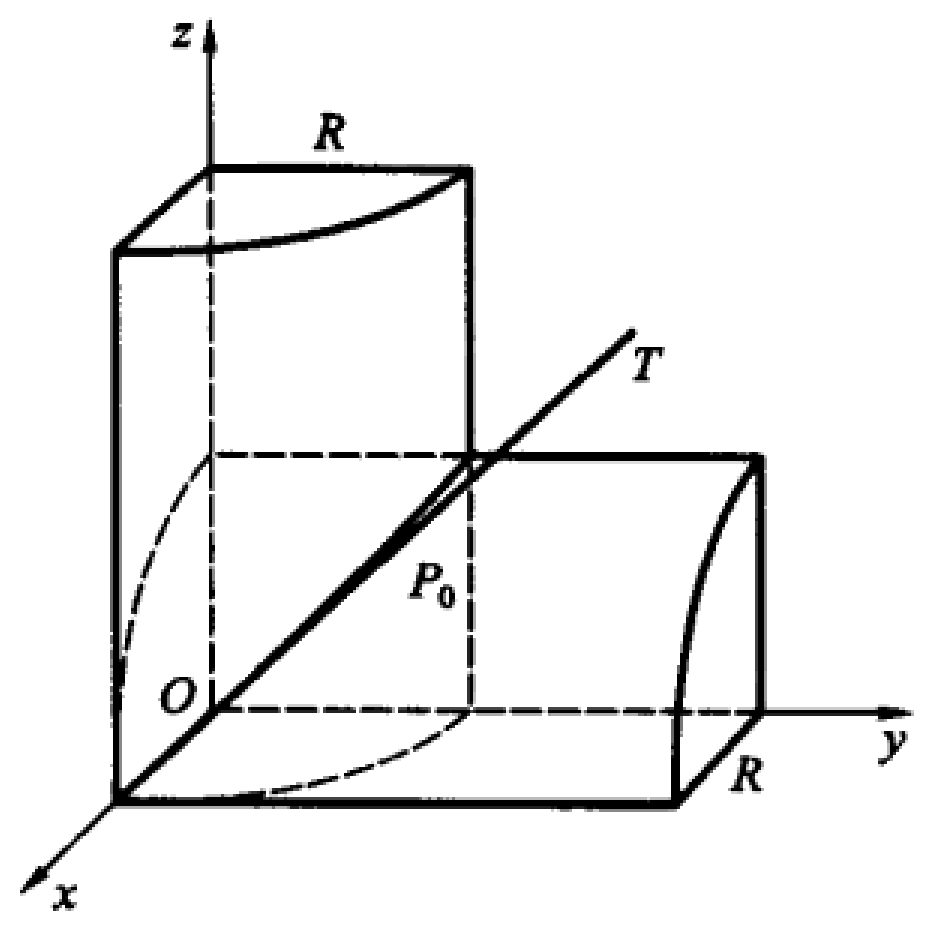
\includegraphics[width=0.5\textwidth]{work/figures/fig16-6}\caption{\relax}\label{fig:16-6}
\end{figure}

因此曲线在 $\left(\dfrac{R}{\sqrt{2}},\dfrac{R}{\sqrt{2}},\dfrac{R}{\sqrt{2}}\right)$ 处的切向量为
\[
\begin{aligned}
\bm{\tau}&=\left.(yz,-xz,-xy)\right|_{\left(\frac{R}{\sqrt{2}},\frac{R}{\sqrt{2}},\frac{R}{\sqrt{2}}\right)}\\
&=\frac{R^{2}}{2}(1,-1,-1),
\end{aligned}
\]
故曲线在 $\left(\dfrac{R}{\sqrt{2}},\dfrac{R}{\sqrt{2}},\dfrac{R}{\sqrt{2}}\right)$ 的切线方程为
\[
x-\frac{R}{\sqrt{2}}=\frac{y-\dfrac{R}{\sqrt{2}}}{-1}=\frac{z-\dfrac{R}{\sqrt{2}}}{-1},
\]
即
\[
\frac{R}{\sqrt{2}}-x=y-\frac{R}{\sqrt{2}}=z-\frac{R}{\sqrt{2}},
\]
而法平面方程为
\[
\left(x-\frac{R}{\sqrt{2}}\right)-\left(y-\frac{R}{\sqrt{2}}\right)-\left(z-\frac{R}{\sqrt{2}}\right)=0,
\]
即
\[
x-y-z+\frac{R}{\sqrt{2}}=0.
\]
\end{proof}

\subsection{空间曲面的切平面与法线}

求空间曲面的切平面与法线，关键在于求切平面的法向量 $\bm{n}$．若已知曲面上一点 $P(x_{0},y_{0},z_{0})$ 处切平面的法向量为
\[
\bm{n}=(A^{\prime},B^{\prime},C^{\prime}),
\]
则曲面在该点的切平面方程为
\[
A^{\prime}(x-x_{0})+B^{\prime}(y-y_{0})+C^{\prime}(z-z_{0})=0.
\]
曲面在该点的法线方程为
\[
\frac{x-x_{0}}{A^{\prime}}=\frac{y-y_{0}}{B^{\prime}}=\frac{z-z_{0}}{C^{\prime}}.
\]
因此下面我们只讨论如何求曲面的法向量 $\bm{n}$．

设曲面方程为
\[
\pi\colon F(x,y,z)=0.
\]
在曲面上任取一条过 $P$ 点的曲线，设其方程为
\[
x=x(t),\ y=y(t),\ z=z(t),
\]
这时有
\[
F(x(t),y(t),z(t))=0.
\]
设 $t=t_{0}$ 对应于点 $P(x_{0},y_{0},z_{0})$，由复合函数求导法，两边对 $t$ 求导并令 $t=t_{0}$，得
\[
F_{x}(x_{0},y_{0},z_{0})x^{\prime}(t_{0})+F_{y}(x_{0},y_{0},z_{0})y^{\prime}(t_{0})+F_{z}(x_{0},y_{0},z_{0})z^{\prime}(t_{0})=0.
\]
写成向量的内积形式
\[
(F_{x},F_{y},F_{z})_{P}\cdot(x^{\prime}(t_{0}),y^{\prime}(t_{0}),z^{\prime}(t_{0}))=0.
\]
上式表明向量 $(F_{x},F_{y},F_{z})_{P}$ 与曲面上任一过 $P$ 点的曲线在 $P$ 点的切线垂直，因此这些切线在同一平面上，这平面就是曲面在 $P$ 点的切平面，而这个切平面的法向量就是
\begin{equation}
\bm{n}=\pm(F_{x},F_{y},F_{z})_{P},
\tag{4}
\end{equation}
它也称为曲面在 $P$ 的法向量．

特别地，若曲面方程为
\[
\pi\colon z=f(x,y),
\]
则只要令
\[
F(x,y,z)=f(x,y)-z,
\]
由（4）式即得曲面在 $P$ 点的法向量为
\begin{equation}
\bm{n}=\pm\left(f_{x},f_{y},-1\right)_{(x_{0},y_{0},z_{0})}.
\tag{5}
\end{equation}

最后，设曲面由参数方程给出
\[
\pi\colon\begin{cases}
x=x(u,v),\\
y=y(u,v),\\
z=z(u,v).
\end{cases}
\]
当 $(u,v)=(u_{0},v_{0})$ 时对应曲面上的点 $P(x_{0},y_{0},z_{0})$．若方程组 $x=x(u,v)$，$y=y(u,v)$ 可确定函数组 $u=u(x,y)$，$v=v(x,y)$，满足 $u_{0}=u(x_{0},y_{0})$，$v_{0}=v(x_{0},y_{0})$，代入 $z=z(u,v)$，则 $z$ 是 $x$、$y$ 的函数 $z=z(u(x,y),v(x,y))$ 且 $z_{0}=z(u(x_{0},y_{0}),v(x_{0},y_{0}))$．于是由（5）式，只要求出 $\left.\dfrac{\partial z}{\partial x}\right|_{P}$ 和 $\left.\dfrac{\partial z}{\partial y}\right|_{P}$ 便可得曲面在 $P$ 点的法向量．为此，我们用隐函数求导法求 $z=z(u,v)$ 对 $u$，$v$ 的偏导数，得
\[
\begin{cases}
\dfrac{\partial z}{\partial u}=\dfrac{\partial z}{\partial x}\dfrac{\partial x}{\partial u}+\dfrac{\partial z}{\partial y}\dfrac{\partial y}{\partial u},\\[8pt]
\dfrac{\partial z}{\partial v}=\dfrac{\partial z}{\partial x}\dfrac{\partial x}{\partial v}+\dfrac{\partial z}{\partial y}\dfrac{\partial y}{\partial v},
\end{cases}
\]
这是关于 $\dfrac{\partial z}{\partial x}$，$\dfrac{\partial z}{\partial y}$ 的线性方程组，当雅可比行列式 $\left.\dfrac{\partial(x,y)}{\partial(u,v)}\right|_{P}\neq 0$ 时，由克拉默法则解得
\[
\left.\frac{\partial z}{\partial x}\right|_{P}=-\left.\frac{\dfrac{\partial(y,z)}{\partial(u,v)}}{\dfrac{\partial(x,y)}{\partial(u,v)}}\right|_{P},\quad \left.\frac{\partial z}{\partial y}\right|_{P}=-\left.\frac{\dfrac{\partial(z,x)}{\partial(u,v)}}{\dfrac{\partial(x,y)}{\partial(u,v)}}\right|_{P}.
\]
代入（5）式并消去公共因子，即得曲面在 $P$ 点的法向量
\begin{equation}
\bm{n}=\pm\left(\frac{\partial(y,z)}{\partial(u,v)},\frac{\partial(z,x)}{\partial(u,v)},\frac{\partial(x,y)}{\partial(u,v)}\right)\bigg|_{P}.
\tag{6}
\end{equation}

\begin{example}\label{ex:16-3-2}
求椭球面 $x^{2}+2y^{2}+3z^{2}=6$ 在 $(1,1,1)$ 点的切平面方程与法线方程．
\end{example}

\begin{proof}[解]
令 $F(x,y,z)=x^{2}+2y^{2}+3z^{2}-6$，则
\[
\begin{aligned}
\bm{n}&=\left.(F_{x},F_{y},F_{z})\right|_{(1,1,1)}\\
&=\left.(2x,4y,6z)\right|_{(1,1,1)}\\
&=2(1,2,3),
\end{aligned}
\]
故所求的切平面方程为
\[
(x-1)+2(y-1)+3(z-1)=0,
\]
即
\[
x+2y+3z-6=0,
\]
而法线方程为
\[
\frac{x-1}{1}=\frac{y-1}{2}=\frac{z-1}{3}.
\]
\end{proof}

\begin{example}\label{ex:16-3-3}
求球面
\[
\begin{cases}
x=\cos\theta\sin\varphi,\\
y=\sin\theta\sin\varphi,\\
z=\cos\varphi
\end{cases}
\]
在对应于 $\theta=\varphi=\dfrac{\pi}{4}$ 处的切平面方程和法线方程．
\end{example}

\begin{proof}[解]
用公式（6）．由
\[
\begin{pmatrix}\dfrac{\partial x}{\partial\theta}&\dfrac{\partial y}{\partial\theta}&\dfrac{\partial z}{\partial\theta}\\[6pt]
\dfrac{\partial x}{\partial\varphi}&\dfrac{\partial y}{\partial\varphi}&\dfrac{\partial z}{\partial\varphi}\end{pmatrix}=\begin{pmatrix}-\sin\theta\sin\varphi&\cos\theta\sin\varphi&0\\ \cos\theta\cos\varphi&\sin\theta\cos\varphi&-\sin\varphi\end{pmatrix},
\]
知
\[
\left.\frac{\partial(y,z)}{\partial(\theta,\varphi)}\right|_{\left(\frac{\pi}{4},\frac{\pi}{4}\right)}=\left.-\cos\theta\sin^{2}\varphi\right|_{\left(\frac{\pi}{4},\frac{\pi}{4}\right)}=-\frac{\sqrt{2}}{4},
\]
\[
\left.\frac{\partial(z,x)}{\partial(\theta,\varphi)}\right|_{\left(\frac{\pi}{4},\frac{\pi}{4}\right)}=\left.-\sin\theta\sin^{2}\varphi\right|_{\left(\frac{\pi}{4},\frac{\pi}{4}\right)}=-\frac{\sqrt{2}}{4},
\]
\[
\left.\frac{\partial(x,y)}{\partial(\theta,\varphi)}\right|_{\left(\frac{\pi}{4},\frac{\pi}{4}\right)}=\left.-\sin\varphi\cos\varphi\right|_{\left(\frac{\pi}{4},\frac{\pi}{4}\right)}=-\frac{1}{2},
\]
从而
\[
\bm{n}=-\frac{\sqrt{2}}{4}(1,1,\sqrt{2}).
\]
又 $\theta=\varphi=\dfrac{\pi}{4}$ 时 $(x,y,z)=\left(\dfrac{1}{2},\dfrac{1}{2},\dfrac{\sqrt{2}}{2}\right)$，故所求的切平面方程为
\[
\left(x-\frac{1}{2}\right)+\left(y-\frac{1}{2}\right)+\sqrt{2}\left(z-\frac{\sqrt{2}}{2}\right)=0,
\]
即
\[
x+y+\sqrt{2}z-2=0,
\]
而法线方程为
\[
x-\frac{1}{2}=y-\frac{1}{2}=\frac{1}{\sqrt{2}}\left(z-\frac{\sqrt{2}}{2}\right).
\]
\end{proof}

\begin{xiti}
\item 求下列曲线在所示点处的切线方程和法平面方程：
\begin{ziti}
\item $x=a\sin^{2}t$，$y=b\sin t\cos t$，$z=c\cos^{2}t$，在点 $t=\dfrac{\pi}{4}$；
\item $2x^{2}+3y^{2}+z^{2}=9$，$z^{2}=3x^{2}+y^{2}$，在点 $(1,-1,2)$；
\item $x^{2}+y^{2}+z^{2}=6$，$x+y+z=0$，在点 $(1,-2,1)$；
\item $x=t-\cos t$，$y=3+\sin^{2}t$，$z=1+\cos 3t$，在点 $t=\dfrac{\pi}{2}$．
\end{ziti}
\item 求下列曲面在所示点处的切平面方程和法线方程：
\begin{ziti}
\item $y-\mathrm{e}^{2x-z}=0$，在点 $(1,1,2)$；
\item $\dfrac{x^{2}}{a^{2}}+\dfrac{y^{2}}{b^{2}}+\dfrac{z^{2}}{c^{2}}=1$ 在点 $\left(\dfrac{a}{\sqrt{3}},\dfrac{b}{\sqrt{3}},\dfrac{c}{\sqrt{3}}\right)$；
\item $z=2x^{2}+4y^{2}$ 在点 $(2,1,12)$；
\item $x=u\cos v$，$y=u\sin v$，$z=av$ 在点 $P_{0}(u_{0},v_{0})$．
\end{ziti}
\item 证明曲线 $x=a\mathrm{e}^{t}\cos t$，$y=a\mathrm{e}^{t}\sin t$，$z=a\mathrm{e}^{t}$ 与锥面 $x^{2}+y^{2}=z^{2}$ 的母线相交成同一角度．
\item 求平面曲线 $x^{2/3}+y^{2/3}=a^{2/3}$ $(a>0)$ 上任一点处的切线方程，并证明这些切线被坐标轴所截取的线段等长．
\item 求曲面 $x^{2}+2y^{2}+3z^{2}=21$ 的切平面，使它平行于平面 $x+4y+6z=0$．
\item 证明：曲面 $F(x-az,y-bz)=0$ 的切平面与某一定直线平行，其中 $a$，$b$ 为常数．
\item 证明曲面 $z=x\mathrm{e}^{\frac{x}{y}}$ 的每一切平面都通过原点．
\item 求两曲面
\[
F(x,y,z)=0,\quad G(x,y,z)=0
\]
的交线在 $Oxy$ 平面上的投影曲线的切线方程．
\end{xiti}

\section{方向导数}

我们已经知道，偏导数给出的是函数沿坐标轴方向的变化率．然而许多实际问题中常常希望知道函数沿任意方向的变化率．例如热量的传导、空气的流动、气压的改变等，沿各个方向的变化率一般是不一样的．下面我们仿照偏导数的定义，引出方向导数的概念．

设函数 $u=f(x,y,z)$，其定义域是空间某区域．在定义域中任取点 $P_{0}(x_{0},y_{0},z_{0})$，由偏导数的定义知，函数 $u$ 在 $P_{0}$ 点关于 $x$ 的偏导数定义为
\[
\left.\frac{\partial u}{\partial x}\right|_{P_{0}}=\lim_{\Delta x\to 0}\frac{f(x_{0}+\Delta x,y_{0},z_{0})-f(x_{0},y_{0},z_{0})}{\Delta x}.
\]
考虑 $\Delta x>0$，并记 $P=(x_{0}+\Delta x,y_{0},z_{0})$，这时 $\Delta x$ 就是 $P$ 与 $P_{0}$ 点的距离 $r(P,P_{0})$．于是上面的极限可用点 $P$ 和 $P_{0}$ 表示为
\[
\lim_{r(P,P_{0})\to 0}\frac{f(P)-f(P_{0})}{r(P,P_{0})}.
\]
注意这里 $P$ 点是始于 $P_{0}$ 点且与 $x$ 轴同方向的射线上的点．如果将 $P$ 点限制在始于 $P_{0}$ 点的另一射线上的点，便得到方向导数的定义．

\begin{figure}[htbp]
\centering
\begin{tikzpicture}[baseline=(current bounding box.center)]
  \coordinate (O) at (0.95,0.05);
  \coordinate (P0) at (1.7,2.3);
  \coordinate (Px) at (0.95,1.8);
  \coordinate (Py) at (3.2,2.3);
  \coordinate (P) at (2.55,1.8);
  \coordinate (B) at (1.7,1.4);
  \coordinate (Bx) at (0.95,0.9);
  \coordinate (By) at (3.2,1.4);
  \coordinate (Bxy) at (2.55,0.9);
  \draw[thick,{-Latex}] (O) -- (0.95,3.2) node[above] {$z$};
  \draw[thick,{-Latex}] (O) -- (3.7,0.05) node[right] {$y$};
  \draw[thick,{-Latex}] (O) -- (0.2,-0.55) node[below] {$x$};
  \node[above left] at (0.9,0.02) {$O$};
  \draw[dashed] (P0) -- (Py) -- (P) -- (Px) -- cycle;
  \draw[dashed] (B) -- (By) -- (Bxy) -- (Bx) -- cycle;
  \draw[dashed] (P0) -- (B) (Py) -- (By) (P) -- (Bxy) (Px) -- (Bx);
  \draw[thick,{-Latex}] (P0) -- (3.45,1.27) node[right] {$\bm{l}$};
  \fill (P0) circle (1.3pt) node[above left] {$P_{0}$};
  \fill (P) circle (1.3pt) node[above right] {$P$};
  \node[left] at (1.66,1.85) {$\Delta z$};
  \node[below left] at (1.32,1.12) {$\Delta x$};
  \node[below] at (1.75,0.9) {$\Delta y$};
\end{tikzpicture}\caption{\relax}\label{fig:16-7}
\end{figure}

\begin{definition}\label{def:16-3}
设三元函数 $u=f(x,y,z)$ 在点 $P_{0}(x_{0},y_{0},z_{0})$ 的某邻域内有定义，任意给定始于点 $P_{0}$ 的射线 $\bm{l}$，$P(x,y,z)$ 为 $\bm{l}$ 上且含于定义域内的点．若极限
\[
\lim_{r(P,P_{0})\to 0^{+}}\frac{f(P)-f(P_{0})}{r(P,P_{0})}=\lim_{r(P,P_{0})\to 0^{+}}\frac{\Delta_{l}f(P_{0})}{r(P,P_{0})}
\]
存在，则称该极限值为函数 $f$ 在点 $P_{0}$ 沿方向 $\bm{l}$ 的方向导数，记为 $\left.\dfrac{\partial f}{\partial l}\right|_{P_{0}}$ 或
\[
\frac{\partial f(P_{0})}{\partial l}.
\]
\end{definition}

$\Delta_{l}f(P_{0})$ 称为函数在 $P_{0}$ 点沿 $\bm{l}$ 方向的增量．若 $\bm{l}$ 的方向余弦为
\[
\bm{l}_{0}=(\cos\alpha,\cos\beta,\cos\gamma),
\]
$P$ 点为 $(x_{0}+\Delta x,y_{0}+\Delta y,z_{0}+\Delta z)$，这时 $\Delta x$，$\Delta y$，$\Delta z$ 不是独立的，它们满足
\[
\frac{\Delta x}{\cos\alpha}=\frac{\Delta y}{\cos\beta}=\frac{\Delta z}{\cos\gamma},
\]
或
\[
\begin{aligned}
\bm{l}_{0}&=(\cos\alpha,\cos\beta,\cos\gamma)\\
&=\frac{1}{\rho}(\Delta x,\Delta y,\Delta z),
\end{aligned}
\]
其中
\[
\rho=r(P,P_{0})=\sqrt{(\Delta x)^{2}+(\Delta y)^{2}+(\Delta z)^{2}}.
\]
当 $\Delta y=\Delta z=0$ 时，$\bm{l}$ 的方向即为 $x$ 轴的正向 $(\Delta x>0)$ 或负向 $(\Delta x<0)$．若 $\Delta x>0$，则
\[
\frac{\partial f(P_{0})}{\partial l}=\frac{\partial f(P_{0})}{\partial x}.
\]
即 $\dfrac{\partial f(P_{0})}{\partial x}$ 就是函数在 $P_{0}$ 点沿 $x$ 轴正向的方向导数．同理 $\dfrac{\partial f(P_{0})}{\partial y}$，$\dfrac{\partial f(P_{0})}{\partial z}$ 分别是函数在 $P_{0}$ 点的沿 $y$ 轴和 $z$ 轴正方向的方向导数．

下面的定理提供了方向导数的简便计算方法．

\begin{theorem}\label{thm:16-6}
若函数 $f(x,y,z)$ 在点 $P_{0}(x_{0},y_{0},z_{0})$ 可微，则 $f(x,y,z)$ 在点 $P_{0}$ 沿任何方向 $\bm{l}$ 的方向导数都存在，且有以下公式
\[
\frac{\partial f(P_{0})}{\partial l}=\frac{\partial f(P_{0})}{\partial x}\cos\alpha+\frac{\partial f(P_{0})}{\partial y}\cos\beta+\frac{\partial f(P_{0})}{\partial z}\cos\gamma.
\]
其中 $\cos\alpha,\cos\beta,\cos\gamma$ 是 $\bm{l}$ 的方向余弦．
\end{theorem}

\begin{proof}
设 $P(x,y,z)$ 是射线 $\bm{l}$ 上的任一点，则
\[
\begin{cases}
x-x_{0}=\Delta x=\rho\cos\alpha,\\
y-y_{0}=\Delta y=\rho\cos\beta,\\
z-z_{0}=\Delta z=\rho\cos\gamma.
\end{cases}
\]
$\rho=\sqrt{(\Delta x)^{2}+(\Delta y)^{2}+(\Delta z)^{2}}$．由于函数 $f(x,y,z)$ 在 $P_{0}(x_{0},y_{0},z_{0})$ 可微，由定义有
\[
f(P)-f(P_{0})=\frac{\partial f(P_{0})}{\partial x}\Delta x+\frac{\partial f(P_{0})}{\partial y}\Delta y+\frac{\partial f(P_{0})}{\partial z}\Delta z+o(\rho)
\]
对任意 $\Delta x$，$\Delta y$，$\Delta z$ 都成立，特别对满足上述关系的 $\Delta x$，$\Delta y$，$\Delta z$ 有
\[
\begin{aligned}
\frac{f(P)-f(P_{0})}{\rho}&=\frac{\partial f(P_{0})}{\partial x}\frac{\Delta x}{\rho}+\frac{\partial f(P_{0})}{\partial y}\frac{\Delta y}{\rho}+\frac{\partial f(P_{0})}{\partial z}\frac{\Delta z}{\rho}+\frac{o(\rho)}{\rho}\\
&=\frac{\partial f(P_{0})}{\partial x}\cos\alpha+\frac{\partial f(P_{0})}{\partial y}\cos\beta+\frac{\partial f(P_{0})}{\partial z}\cos\gamma+\frac{o(\rho)}{\rho}.
\end{aligned}
\]
令 $\rho\to 0$ 取极限即得
\[
\frac{\partial f(P_{0})}{\partial l}=\frac{\partial f(P_{0})}{\partial x}\cos\alpha+\frac{\partial f(P_{0})}{\partial y}\cos\beta+\frac{\partial f(P_{0})}{\partial z}\cos\gamma.
\]
定理~\ref{thm:16-6} 证完．
\end{proof}

定理中的公式又可用矢量的内积表示为
\[
\frac{\partial f(P_{0})}{\partial l}=\left(\frac{\partial f}{\partial x},\frac{\partial f}{\partial y},\frac{\partial f}{\partial z}\right)\bigg|_{P_{0}}\cdot(\cos\alpha,\cos\beta,\cos\gamma).
\]

对于二元函数 $u=f(x,y)$，它在 $P_{0}(x_{0},y_{0})$ 点沿任一方向 $\bm{l}=(\cos\alpha,\cos\beta)$ 的方向导数为
\[
\begin{aligned}
\frac{\partial f(x_{0},y_{0})}{\partial l}&=\frac{\partial f(x_{0},y_{0})}{\partial x}\cos\alpha+\frac{\partial f(x_{0},y_{0})}{\partial y}\cos\beta\\
&=\left(\frac{\partial f}{\partial x},\frac{\partial f}{\partial y}\right)\bigg|_{(x_{0},y_{0})}\cdot(\cos\alpha,\cos\beta).
\end{aligned}
\]

\begin{example}\label{ex:16-4-1}
求函数 $u=xy^{2}+z^{3}-xyz$ 在点 $(1,1,2)$ 处沿方向 $\bm{l}$ 的方向导数，$\bm{l}$ 的方向角分别为 $60^{\circ}$，$45^{\circ}$，$60^{\circ}$．
\end{example}

\begin{proof}[解]
$\bm{l}$ 的方向余弦为
\[
(\cos 60^{\circ},\cos 45^{\circ},\cos 60^{\circ})=\left(\frac{1}{2},\frac{\sqrt{2}}{2},\frac{1}{2}\right).
\]
又
\[
\begin{aligned}
&\left(\frac{\partial u}{\partial x},\frac{\partial u}{\partial y},\frac{\partial u}{\partial z}\right)\bigg|_{(1,1,2)}\\
&=\left(y^{2}-yz,2xy-xz,3z^{2}-xy\right)|_{(1,1,2)}\\
&=(-1,0,11).
\end{aligned}
\]
故
\[
\left.\frac{\partial u}{\partial l}\right|_{(1,1,2)}=(-1,0,11)\cdot\left(\frac{1}{2},\frac{\sqrt{2}}{2},\frac{1}{2}\right)=5.
\]
\end{proof}

\begin{xiti}
\item 设 $f(x,y,z)=x+y^{2}+z^{3}$，求 $f$ 在点 $P_{0}(1,1,1)$ 沿方向 $\bm{l}=(2,-2,1)$ 的方向导数．
\item 求函数 $u=xyz$ 在点 $A(5,1,2)$ 处沿到点 $B(9,4,14)$ 的方向 $\overrightarrow{AB}$ 上的方向导数．
\item 求 $\left.\dfrac{\partial u}{\partial l}\right|_{(x_{0},y_{0})}$：
\begin{ziti}
\item $u=\ln\left(x^{2}+y^{2}\right)$，$(x_{0},y_{0})=(1,1)$，$\bm{l}$ 与 $x$ 轴正向的夹角为 $60^{\circ}$；
\item $u=x\mathrm{e}^{xy}$，$(x_{0},y_{0})=(1,1)$，$\bm{l}$ 与向量 $(1,1)$ 同向．
\end{ziti}
\item 设函数 $f(x,y)$ 在 $(x_{0},y_{0})$ 可微，单位向量 $\bm{l}_{1}=\left(\dfrac{1}{\sqrt{2}},\dfrac{1}{\sqrt{2}}\right)$，$\bm{l}_{2}=\left(-\dfrac{1}{\sqrt{2}},\dfrac{1}{\sqrt{2}}\right)$，$\dfrac{\partial f(x_{0},y_{0})}{\partial l_{1}}=1$，$\dfrac{\partial f(x_{0},y_{0})}{\partial l_{2}}=0$，确定 $\bm{l}$ 使得
\[
\frac{\partial f(x_{0},y_{0})}{\partial l}=\frac{7}{5\sqrt{2}}.
\]
\item 设 $f$ 在 $P_{0}(2,0)$ 可微，$f(x,y)$ 在 $P_{0}$ 指向 $P_{1}=(2,-2)$ 的方向导数是 $1$，指向原点的方向导数是 $-3$，试回答：
\begin{ziti}
\item 指向 $P_{2}=(2,1)$ 的方向导数是多少？
\item 指向 $P_{3}=(3,2)$ 的方向导数是多少？
\end{ziti}
\end{xiti}

\section{泰勒公式}

回忆一元函数的泰勒公式：若 $f(x)$ 在 $x_{0}$ 点的某邻域有 $n+1$ 阶连续微商，则当 $x=x_{0}+\Delta x$ 属于该邻域时，有
\begin{equation}
f\left(x_{0}+\Delta x\right)=\sum_{k=0}^{n}\frac{f^{(k)}\left(x_{0}\right)}{k!}\Delta x^{k}+R_{n}(x).
\tag{1}
\end{equation}
其中 $R_{n}(x)$ 可用拉格朗日余项形式表出
\[
R_{n}(x)=\frac{1}{(n+1)!}f^{(n+1)}\left(x_{0}+\theta\Delta x\right)\Delta x^{n+1},\quad 0<\theta<1.
\]

对于二元函数，有类似的结果成立．

\begin{theorem}[（泰勒定理）]\label{thm:16-7}
设 $f(x,y)$ 在 $P_{0}(x_{0},y_{0})$ 的某邻域 $O(P_{0})$ 内有直到 $n+1$ 阶连续偏导数，则对 $O(P_{0})$ 内任一点 $(x_{0}+\Delta x,y_{0}+\Delta y)$，存在 $\theta\in(0,1)$，使得
\begin{equation}
f\left(x_{0}+\Delta x,y_{0}+\Delta y\right)=\sum_{k=0}^{n}\frac{1}{k!}\left(\frac{\partial}{\partial x}\Delta x+\frac{\partial}{\partial y}\Delta y\right)^{k}f\left(x_{0},y_{0}\right)+R_{n},
\tag{2}
\end{equation}
其中
\[
R_{n}=\frac{1}{(n+1)!}\left(\frac{\partial}{\partial x}\Delta x+\frac{\partial}{\partial y}\Delta y\right)^{n+1}f\left(x_{0}+\theta\Delta x,y_{0}+\theta\Delta y\right).
\]
\end{theorem}

\begin{proof}
用一元函数的结果．引入参数 $t$，构造函数
\[
\varphi(t)=f\left(x_{0}+t\Delta x,y_{0}+t\Delta y\right),\quad t\in[0,1].
\]
这时 $\varphi(0)=f(x_{0},y_{0})$，$\varphi(1)=f(x_{0}+\Delta x,y_{0}+\Delta y)$．由 $f(x,y)$ 在 $O(P_{0})$ 内有直到 $n+1$ 阶连续偏导数，知复合函数 $\varphi(t)$ 在 $[0,1]$ 有直到 $n+1$ 阶的连续导数，且可用复合函数求导的链式法则求出
\[
\begin{aligned}
\varphi^{(k)}(t)&=\left(\frac{\partial}{\partial x}\Delta x+\frac{\partial}{\partial y}\Delta y\right)^{k}f\left(x_{0}+t\Delta x,y_{0}+t\Delta y\right),\\
&&k=1,2,\cdots,n+1.
\end{aligned}
\]
由一元函数拉格朗日型余项的泰勒公式，存在 $\theta\in(0,1)$，使得
\[
\varphi(1)=\sum_{k=0}^{n}\frac{\varphi^{(k)}(0)}{k!}+\frac{1}{(n+1)!}\varphi^{(n+1)}(\theta),
\]
即
\[
\begin{aligned}
&f\left(x_{0}+\Delta x,y_{0}+\Delta y\right)\\
={}&\sum_{k=0}^{n}\frac{1}{k!}\left(\frac{\partial}{\partial x}\Delta x+\frac{\partial}{\partial y}\Delta y\right)^{k}f\left(x_{0},y_{0}\right)+{}\\
&\frac{1}{(n+1)!}\left(\frac{\partial}{\partial x}\Delta x+\frac{\partial}{\partial y}\Delta y\right)^{n+1}f\left(x_{0}+\theta\Delta x,y_{0}+\theta\Delta y\right).
\end{aligned}
\]
定理~\ref{thm:16-7} 证完．
\end{proof}

公式 (2) 称为二元函数 $f(x,y)$ 在 $(x_{0},y_{0})$ 点的 $n$ 阶泰勒公式．式中的余项 $R_{n}$ 称为拉格朗日型余项．当 $n=0$ 时，就得到二元函数的中值公式：
\begin{equation}
\begin{aligned}
&f\left(x_{0}+\Delta x,y_{0}+\Delta y\right)-f\left(x_{0},y_{0}\right)\\
=\;&f_{x}\left(x_{0}+\theta\Delta x,y_{0}+\theta\Delta y\right)\Delta x+f_{y}\left(x_{0}+\theta\Delta x,y_{0}+\theta\Delta y\right)\Delta y,\\
&&0<\theta<1.
\end{aligned}
\tag{3}
\end{equation}

下面我们忽略余项，把 $n=0,1,2$ 的泰勒展开式写出来．
\[
\begin{aligned}
n=0,\qquad&f\left(x_{0}+\Delta x,y_{0}+\Delta y\right)\approx f\left(x_{0},y_{0}\right)\\
n=1,\qquad&f\left(x_{0}+\Delta x,y_{0}+\Delta y\right)\\
\approx\;&f\left(x_{0},y_{0}\right)+f_{x}\left(x_{0},y_{0}\right)\Delta x+f_{y}\left(x_{0},y_{0}\right)\Delta y,\\
n=2,\qquad&f\left(x_{0}+\Delta x,y_{0}+\Delta y\right)\\
\approx\;&f\left(x_{0},y_{0}\right)+f_{x}\left(x_{0},y_{0}\right)\Delta x+f_{y}\left(x_{0},y_{0}\right)\Delta y+\\
&\frac{1}{2}\left\{f_{xx}\left(x_{0},y_{0}\right)\Delta x^{2}+2f_{xy}\left(x_{0},y_{0}\right)\Delta x\Delta y+f_{yy}\left(x_{0},y_{0}\right)\Delta y^{2}\right\}.
\end{aligned}
\]
$n=1$ 时，正是用函数的微分代替函数的改变量．

\begin{example}\label{ex:16-5-1}
设 $f(x,y)=x^{y}$，利用 $f(x,y)$ 在点 $(1,4)$ 的二阶泰勒公式，近似计算 $(1.08)^{3.96}$．
\end{example}

\begin{proof}[解]
\[
\begin{aligned}
&f(x,y)=x^{y},\qquad\qquad\qquad\qquad\ \ f(1,4)=1\,;\\
&f_{x}(x,y)=yx^{y-1},\qquad\qquad\qquad\ \ f_{x}(1,4)=4\,;\\
&f_{y}(x,y)=x^{y}\ln x,\qquad\qquad\qquad\ \ f_{y}(1,4)=0\,;\\
&f_{x^{2}}(x,y)=y(y-1)x^{y-2},\qquad\quad f_{x^{2}}(1,4)=12\,;\\
&f_{xy}(x,y)=x^{y-1}+yx^{y-1}\ln x,\qquad\ \ f_{xy}(1,4)=1\,;\\
&f_{y^{2}}(x,y)=x^{y}\ln^{2}x,\qquad\qquad\quad\;\; f_{y^{2}}(1,4)=0.
\end{aligned}
\]
\[
\begin{aligned}
x^{y}\approx\;&f(1,4)+f_{x}(1,4)(x-1)+f_{y}(1,4)(y-4)+\\
&\frac{1}{2!}\left[f_{x^{2}}(1,4)(x-1)^{2}+2f_{xy}(1,4)(x-1)(y-4)+\right.\\
&\left.f_{y^{2}}(1,4)(y-4)^{2}\right]\\
=\;&1+4(x-1)+6(x-1)^{2}+(x-1)(y-4),
\end{aligned}
\]
取 $x=1.08$，$y=3.96$，得
\[
\begin{aligned}
1.08^{3.96}&\approx 1+4\times 0.08+6\times 0.08^{2}+0.08(-0.04)\\
&=1.355\ 2.
\end{aligned}
\]
\end{proof}

在本章 §1 中，我们曾用全微分近似函数的改变量，或说用一阶多项式逼近函数 $f(x,y)$，计算过 $1.08^{3.96}$ 的近似值为 $1.08^{3.96}\approx 1.32$．现在我们是用二阶多项式逼近函数 $f(x,y)$，得近似值 $1.08^{3.96}\approx 1.355\ 2$，比前面稍为精确了一些．利用泰勒公式，我们还可用 $n$ 阶多项式逼近函数 $f(x,y)$，$n$ 越大则误差越小，近似程度越好．

\begin{xiti}
\item 写出下列函数在指定点的泰勒公式：
\begin{ziti}
\item $f(x,y)=2x^{2}-xy-y^{2}-6x-3y+5$，在 $(1,-2)$ 点；
\item $f(x,y)=x^{2}+xy+y^{2}+3x-2y+4$，在 $(-1,1)$ 点．
\end{ziti}
\item 求函数 $f(x,y)=\dfrac{x}{y}$ 在 $(1,1)$ 点邻域的 $n$ 阶带拉格朗日余项的泰勒公式．
\item 求函数 $f(x,y)=\dfrac{y^{2}}{x^{2}}$ 在 $(1,-1)$ 点邻域的二阶泰勒公式，并写出拉格朗日余项．
\item 求下列函数在 $(0,0)$ 点邻域的四阶泰勒公式：
\begin{ziti}
\item $f(x,y)=\sin\left(x^{2}+y^{2}\right)$；
\item $f(x,y)=\mathrm{e}^{x}\ln(1+y)$；
\item $f(x,y)=\sqrt{1+x^{2}+y^{2}}$；
\item $f(x,y)=\mathrm{e}^{x}\cos y$．
\end{ziti}
\item 证明泰勒公式的唯一性：若
\[
\sum_{i+j=0}^{n}A_{ij}x^{i}y^{j}+o\left(\rho^{n}\right)=0\quad(\rho\to 0),
\]
其中 $\rho=\sqrt{x^{2}+y^{2}}$．求证 $A_{ij}=0$（$i,j$ 为非负整数，$i+j=0,1,\cdots,n$），并利用唯一性求 $f(x,y)=\ln(1+x+y)$ 在 $(0,0)$ 点带拉格朗日余项的 $n$ 阶泰勒展开式．
\item 通过对 $f(x,y)=\sin x\cos y$ 用中值定理，证明存在 $\theta\in(0,1)$，使
\[
\frac{3}{4}=\frac{\pi}{3}\cos\frac{\pi\theta}{3}\cos\frac{\pi\theta}{6}-\frac{\pi}{6}\sin\frac{\pi\theta}{3}\sin\frac{\pi\theta}{6}.
\]
\item 设 $f(x,y)$ 在区域 $D$ 内有偏导数存在，且 $f_{x}(x,y)=f_{y}(x,y)\equiv 0$．证明 $f(x,y)$ 在 $D$ 内为常数．
\item 若 $\left|x\right|$，$\left|y\right|$ 是很小的量，导出下列函数准确到二次项的近似公式：
\begin{ziti}
\item $\dfrac{\cos x}{\cos y}$；
\item $\arctan\dfrac{1+x+y}{1-xy}$．
\end{ziti}
\item 设函数 $f(x,y)$ 有直到 $n$ 阶连续偏导数，试证 $u(t)=f(a+ht,b+kt)$ 的 $n$ 阶导数
\[
u^{(n)}(t)=\left(h\frac{\partial}{\partial x}+k\frac{\partial}{\partial y}\right)^{n}f(a+ht,b+kt).
\]
\item 设 $f(x,y)$ 为 $n$ 次齐次函数，证明
\[
\left(x\frac{\partial}{\partial x}+y\frac{\partial}{\partial y}\right)^{m}f=n(n-1)\cdots(n-m+1)f.
\]
\item 设 $f(x,y)=\psi(ax+by)$，其中 $a$，$b$ 为常数，在包含原点的某邻域内，$\psi$ 有 $q$ 阶连续导数．求证：在 $(0,0)$ 点邻域的泰勒公式是
\[
f(x,y)=\sum_{k=0}^{q-1}\frac{\psi^{(k)}(0)}{k!}\sum_{j=0}^{k}\mathrm{C}_{k}^{j}(ax)^{j}(by)^{k-j}+R_{q}(x,y).
\]
\end{xiti}




